%!!!!!!!!!!!!!!!!!!!!!!!!!!!!!!!!!!!!!!!!!!!!!!!!!!!!!!!!!!!!!!!!!!!!!!!!!!!!!!
%!NOTE: This example file has been prepared according to the University of
%!      Hawaii Style & Policy Manual for Theses and Dissertations dated
%!      "Revised September 2010". If you have one with a later date, you may
%!      need to make revisions to this document as well. In any event, making
%!      sure your thesis complies with Graduate Education guidelines is
%!      ultimately your responsibility. Caveat LaTeXtor. :)
%!!!!!!!!!!!!!!!!!!!!!!!!!!!!!!!!!!!!!!!!!!!!!!!!!!!!!!!!!!!!!!!!!!!!!!!!!!!!!!

%% The options are (you can only choose one from each group):
%%
%% 10pt, 11pt, 12pt: chooses the point size for the document. "11pt" is the
%%                   default.
%%
%% oneside, twoside: whether you want your document onesided or twosided. Note
%%                   that twosided is not guaranteed to work, and style
%%                   guidelines prohibit double sided printouts on final
%%                   copy. "oneside" is the default.
%%
%% draft, final: when printing drafts you can save a lot of paper by using the
%%               "draft" option. It switches to single spacing, displays overful
%%               hboxes with a black box, prints a version number on title page 
%%               and omits signature page. Of course for the final copy make
%%               sure to use the "final" option! "final" is the default.
%%
%% thesis, dissertation: switches between the style for a master's thesis and a 
%%                       Ph.D. dissertation. The differences are fairly minor
%%                       and limited to the front matter. "thesis" is the
%%                       default.
%%
%% actual, proposal: switches between actual document and proposal mode. In
%%                   proposal mode: the title page is simplified and the
%%                   version number is always printed.
%%
%%% Load the new uhthesis document class
\documentclass[11pt, dissertation, proposal]{uhthesis}

%%% Load some useful packages:
%% New LaTeX2e graphics support
\usepackage{graphicx}
%% Package to linebreak URLs in a sane manner.
\usepackage{url}

\usepackage{hyperref}

%%% Declarations for Front Matter. Capitalize all of these values
%%% "normally". This allows the document class to format them properly.
%% Full title of thesis or dissertation, capitalized like a title should be.
\title{Laha: a Framework for Adaptive Optimization of Distributed Sensor Frameworks}
%% Your name, capitalized normally. Do not include any titles like Dr.
\author{Anthony J. Christe}
%% Month in which you intend to receive your degree (i.e. graduation).
%% Presumably this will be one of: May, August, or December.
\degreemonth{December}
%% Year of expected graduation.
\degreeyear{2019}
%% Type of degree to be conferred.
\degree{Doctor of Philosophy}
%% This is the chairperson of your committee. Do not use titles like Dr.
\chair{Philip Johnson}
%% The other members of your committee, seperated by "\\". Again, no titles,
%% and it is customary to list the outside committee member (if you have one)
%% last.
\othermembers{Lipyeow Lim\\
Dan Suthers?\\
Peter Sadowski?\\
Milton Garces}
%% The field in which you are obtaining your degree, capitalized normally.
\field{Computer Science}
%% If your discipline allows subfields, you can add it here. Note that this
%% is strictly controlled, so consult the Style & Policy guide before adding
%% a subfield.
%\subfield{Bioinformatics}
%% 4-6 optional keywords/phrases for use in indexing or as search terms
\keywords{distributed, sensors, management, adaptive, optimizing, predictive}
%% The version number of your document. Consistent use of this will enable you
%% to tell old drafts from new ones. Final actual documents omit this
%% automatically so you can use it without fear of submission problems at the
%% end. If you do not define this parameter, it defaults to "1.0.0".
\versionnum{0.6}

%%% End of preamble
\begin{document}
\maketitle

\begin{frontmatter}

%%% Note, there is no longer a signature page included in the document, it
%%% has been replaced by Form IV

%%% Create the copyright page (optional)
\copyrightpage

%%% Bring in the dedication page from external file (optional)
%%%%%%%%%%%%%%%%%%%%%%%%%%%%%%% -*- Mode: Latex -*- %%%%%%%%%%%%%%%%%%%%%%%%%%%%
%% uhtest-dedication.tex -- 
%% Author          : Robert Brewer
%% Created On      : Fri Oct  2 16:29:01 1998
%% Last Modified By: Robert Brewer
%% Last Modified On: Fri Oct  2 16:29:20 1998
%% RCS: $Id: uhtest-dedication.tex,v 1.1 1998/10/06 02:07:25 rbrewer Exp $
%%%%%%%%%%%%%%%%%%%%%%%%%%%%%%%%%%%%%%%%%%%%%%%%%%%%%%%%%%%%%%%%%%%%%%%%%%%%%%%
%%   Copyright (C) 1998 Robert Brewer
%%%%%%%%%%%%%%%%%%%%%%%%%%%%%%%%%%%%%%%%%%%%%%%%%%%%%%%%%%%%%%%%%%%%%%%%%%%%%%%
%% 

\begin{dedication}
\null\vfil
{\large
\begin{center}
To my father. If only you could see me now.
\end{center}}
\vfil\null
\end{dedication}


%%% Bring in the acknowledgments section from external file (optional)
%%%%%%%%%%%%%%%%%%%%%%%%%%%%%%% -*- Mode: Latex -*- %%%%%%%%%%%%%%%%%%%%%%%%%%%%
%% uhtest-acknowledgements.tex -- 
%% Author          : Robert Brewer
%% Created On      : Fri Oct  2 16:29:43 1998
%% Last Modified By: Robert Brewer
%% Last Modified On: Fri Oct  2 16:29:52 1998
%% RCS: $Id: uhtest-acknowledgements.tex,v 1.1 1998/10/06 02:06:54 rbrewer Exp $
%%%%%%%%%%%%%%%%%%%%%%%%%%%%%%%%%%%%%%%%%%%%%%%%%%%%%%%%%%%%%%%%%%%%%%%%%%%%%%%
%%   Copyright (C) 1998 Robert Brewer
%%%%%%%%%%%%%%%%%%%%%%%%%%%%%%%%%%%%%%%%%%%%%%%%%%%%%%%%%%%%%%%%%%%%%%%%%%%%%%%
%% 

\begin{acknowledgments}
To my committee, friends, and family: Thank you for sticking with me through my lengthy academic career. 
\end{acknowledgments}


%%% Bring in the abstract section from external file
%%%%%%%%%%%%%%%%%%%%%%%%%%%%%% -*- Mode: Latex -*- %%%%%%%%%%%%%%%%%%%%%%%%%%%%
%% uhtest-abstract.tex -- 
%% Author          : Robert Brewer
%% Created On      : Fri Oct  2 16:30:18 1998
%% Last Modified By: Robert Brewer
%% Last Modified On: Fri Oct  2 16:30:25 1998
%% RCS: $Id: uhtest-abstract.tex,v 1.1 1998/10/06 02:06:30 rbrewer Exp $
%%%%%%%%%%%%%%%%%%%%%%%%%%%%%%%%%%%%%%%%%%%%%%%%%%%%%%%%%%%%%%%%%%%%%%%%%%%%%%%
%%   Copyright (C) 1998 Robert Brewer
%%%%%%%%%%%%%%%%%%%%%%%%%%%%%%%%%%%%%%%%%%%%%%%%%%%%%%%%%%%%%%%%%%%%%%%%%%%%%%%
%% 

%% Revision notes


\begin{abstract}
I propose an abstract distributed sensor network framework, Laha, that adaptively optimizes triggering, collection, detection, classification, sensor device power requirements, and bandwidth. The Laha data model can be conceptualized as a multilevel pyramid (see fig. \ref{laha-abstract-overview}). Laha Actors act on the data model to move data upward through the levels and to apply optimizations downward through the levels. 

The lowest level stores all recently received raw sensor data. This data expires and is automatically removed within a limited period of time (for example, 1 hour) unless the data is found to be interesting and is thus propagated upwards to the next level of the hierarchy.  Higher levels of the data hierarchy organize data in the same way, however each level adds context to the examined signal or signals. Context includes classifications, locality metrics, temporal metrics, or similarities to current or prior signals of interest. The highest level of the hierarchy, Phenomena, represents predictive capabilities of the sensor network which are then used to optimize and tune the lower levels.

A high level summary of the Laha abstract framework is provided as figure \ref{laha-abstract-overview}. The figure shows the levels and names of the hierarchy, a brief description of the functions of each level, and Laha's Actors and how they move data upwards (right hand side) and how they apply optimizations downwards (left hand side).


\begin{figure}
	\caption{Laha Conceptual Model Summary}
	\centering
	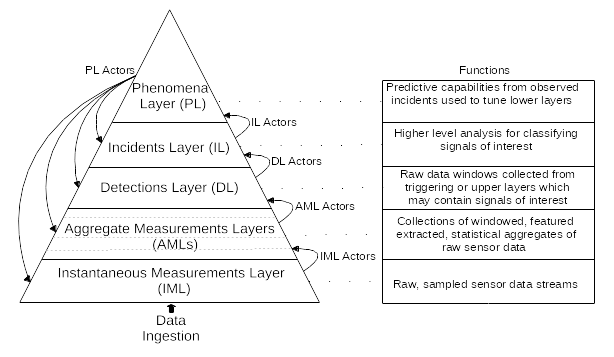
\includegraphics{figures/laha_abstract_overview.png}	
	\label{laha-abstract-overview}
\end{figure}
%Laha's data hierarchy includes the following levels. At each level, we further refine the data which is forwarded to higher layers in the hierarchy and filter out sensor noise. The lowest level, the Instantaneous Measurements Layer (IML) receives raw, sampled data from the network and forwards aggregate measurements to the Aggregate Measurements Layer (AML). The AML consumes feature extracted data streams to provide triggers for possible signals of interest which are forwarded to the Detections Layer (DL). The DL receives raw data from a subset of network sensors corresponding to time windows as determined in the AML. The DL data is forwarded to the Incidents Layer (IL) where standard and state of the art algorithms are used to identify and classify signals of interest within the windows provided by the DL. Finally, data from the DL is forwarded to the Phenomenon Layer (PL) where context, causality, and predictive analytics are created. Phenomena are then used to adaptively tune and optimize the lower levels of the hierarchy.

The Laha framework aims to provide seven useful benefits. Tiered management of Big Data where each tier has configurable time-to-live (TTL) requirements which provides a predicted upper bounds on bandwidth and storage requirements at the cost of potentially discarding important information. Automatically providing context to classified incidents based off of user and algorithmically tagged incidents. Adaptive optimization of triggering within the network to decrease bandwidth and increase accuracy. Adaptive optimizations for detection and classification algorithms power by Laha's Phenomena. Building of a model of the underlying sensor field topology by observing how signals travel and are received across multiple devices. Decreased bandwidth throughout the DSN as result of increased triggering, detection, and classification efficiency. Finally, minimizing of power sensor requirements as a result of increased triggering, detection, and classification efficiency. 

Laha will be evaluated by designing and implementing two Laha-compliant reference implementations, OPQMauka and Lokahi. Open Power Quality (OPQ) is a power quality (PQ) network consisting of custom hardware and distributed software services that detect distributed PQ signals such as voltage sags and swells, frequency sags and swells, transients, THD, and other known PQ issues. OPQMauka is a distributed, plugin based middleware component of OPQ that performs higher level analysis, data management, and optimizations of the OPQ services. Lokahi is a distributed infrasound network consisting of mobile iOS and Android devices and multiple cloud based software services whose purpose is to supplement the International Monitoring System (IMS) in detecting large infrasound signals. 

The reference implementations will be deployed to test sites at UH Manoa and at the Infrasound Laboratory in Kailua-Kona, Big Island. 

Data collected from the PQ network will be validated against calibrated reference sensors that have already been installed at the power mains of a subset of buildings on campus. The Office of Energy Management at UH Manoa has given us full access to live and historic PQ data collected at these reference sensors. OPQBoxes will be co-located and placed in buildings with the reference sensors so that we can validate that the triggering and raw data streams we receive from the OPQBoxes are in line with what the reference sensors are observing. 

Data collected from the infrasound network will also be validated against industry standard calibrated BNK infrasound sensors. Further, signals in the infrasound network are known a priori since I am able to control the signals that are generated from our calibrated infrasound source, allowing further validation of received signals. 

To evaluate the seven benefits from Laha, several different approaches are taken depending on the Laha deployment. In the UH Manoa PQ deployment, we will co-locate sensors in our deployment and for each metric one of the sensors will use Laha's optimizations and the other sensor will not. This will provide metrics that allows us to compare and contrast our optimization techniques within the OPQ network. In the Lokahi infrasound network, we will run a series of experiments where we can produce the same infrasound signals in each experiment and only change the tuning and optimizations that Laha applies to generate metrics for evaluation within the Laha network.

% TODO provide name of industry standard OPQ sensors for validation
% TODO How do we evaluate the data?

I expect to deploy reference implementations before the end of 2018 with validated data collection beginning and continuing through Q3 2019. I anticipate writing my dissertation along side the deployment and data collection process and to be finished in Q3 2019. 

% Proposed contributions
\end{abstract}


%%% Generate table of contents
\tableofcontents

%%% Generate list of tables
\listoftables

%%% Generate list of figures
\listoffigures

\end{frontmatter}

%\normalsize
%%% Bring in the body of the thesis from external file
\chapter{Introduction}

\section{Overview of Distributed Sensor Networks}
Distributed sensor networks (DSNs) consist of any number of sensors that collect and sense information about the physical environment around them. The sensors that make up these networks can either be homogeneous or heterogeneous. Distributed sensor networks are dynamic in that sensors can be added or removed from the network at any time. DSNs also increasingly include mobile sensors as well. With the onset of the Internet of Things (IoT), its easier than ever to build and deploy distributed sensor networks. Further, mobile devices, such as mobile phones, are seeing increased usage as intelligent sensing agents.

\subsection{DSN Data Collection Schemes}
Data can be collected from DSNs in various ways. Sensors can store data onboard to be collected manually or transmit data via a multitude of mediums (satellites, radio, laser, wired connections) using a slew of standards (TCP/IP, Zigbee, Bluetooth, custom, etc).

In some DSNs, data is routed between the sensors using various approaches and eventually makes its way to a sink or sinks. A sink is a data collection node. Cloud computing has become a prevalent choice for DSN sinks since they often provide the ability to provision resources as needed. Various approaches have been proposed that minimize and optimize communications between sensors within a DSN.

In other DSNs, sensor nodes have direct access to a sink, and instead of communicating with each other and passing messages among themselves, the nodes send their data directly to the sink. It's also possible for a DSN to take a hybrid approach and performs some communication within the network and some directly to the sink.

Not only are there various approaches to routing data, but there are also various approaches to deciding what kind of data to send (or acquire).

\subsection{DSN Detection Schemes}
On one extreme end, we have the send everything approach where each sensor sends its data to the sink all the time (or at least when it has the means to do). In this scenario, the sink is responsible for collection, cleaning, detection, and classification of signals and events within the data. This approach can be bandwidth and energy intensive, but provides the benefit of allowing more complete analysis to occur beyond the sink where more computational resources exist. This provides more accurate results and allows the sink to examine the results in aggregate with the rest of the DSN.

The other extreme is that sensors only send data when they have detected a signal of interest. In this scenario, sensors use onboard computing capabilities to filter their sensor stream and perform signal detection on the device. Only when the devices make a detection do they send the detection or data stream to a sink for further processing. This minimizes bandwidth but detection and classification of signals must occur with more constrained computing and energy environments. Further, the global state of the network can't be known without adding the complexity of sensor-to-sensor communication.

Often time a hybrid approach is taken where low fidelity feature extracted and sometimes aggregate data is sent from the sensors to the sink. The sink analyzes the low fidelity feature extracted stream to determine if raw data should be requested from the sensors. The act of requesting data from the sensors is called triggering. This approach is useful because we still gain bandwidth benefits and can easily gain an understanding of the global state of a network.

With all of these factors combined, management, collection, detection, localization, and analysis from distributed sensor networks is not a trivial task. DSNs can produce massive amounts of data. The emergence of IoT has increased the heterogeneity of sensors with multiple hardware configurations, variations of data APIs, and incomplete or bad sensor data. For these reasons, the data collected from distributed sensor networks under certain circumstances is considered Big Data.

\subsection{DSN Classification Schemes}
% TODO

\subsection{DSNs as Big Data}
Big Data is generally defined by the four V's; volume, velocity, variety, and value. These characteristics can be observed in many of the DSNs that exist and are being created today. % TODO more citations

That is, distributed sensor networks create a large volume of data due to the abundance of IoT and mobile devices that make up DSNs. As communication infrastructures improve and hardware becomes smaller, smarter and more energy efficient, sensors are able to send and transfer larger amounts of data. The ease of building and deploying sensors in DSNs means that more sensors can be produced much more cheaply allowing for more sensors to be used within a DSN, increasing coverage, but also increasing the volume of data.

Distributed sensor networks create a variety of data with different formats and data quality issues. Distributed sensor networks can produce data at high velocity. These characteristics of data produced from distributed sensor networks create a need for efficient architectures and specific algorithms designed for working with Big Data.

Further, sensor networks are often constrained in both computing power and available energy sources. This forces us to find comprises between data collection, onboard sensor processing, sensor communication, and network coordination.

This proposal focuses on identifying and tuning several aspects of distributed sensor networks.

Triggering is the act of monitoring low fidelity feature extracted data and triggering sensors for high fidelity data streams when abnormalities are seen in the triggering data stream.

Detection is the algorithmic ability to detect signals of interest among a sea of background noise. Sensor networks often detect signals without knowing what they are or how to classify them.

Classification is the act of associating a signal with a known designation.

\section{The Data Management and Analysis Problems}

\section{Traditional Approaches to Data Management and Analysis}

\section{Seven proposed benefits of Laha} \label{laha-benefits}
Laha is designed to adaptively optimize the collection, triggering, detection, and classification of signals within a DSN. These optimizations provide several benefits to DSNs.

\subsection{Tiered management of Big Data}
% TODO If you're going to use "Big Data" as a term of art, then it needs to be rigorously defined.
Laha provides tiered management of the Big Data that the framework consumes. This is mainly accomplished using the layered approach that Laha provides. All data within the Laha framework is garbage collected using a configurable time to live (TTL) for each layer. As data moves from the bottom to the top of the framework, noise is discarded and only interesting data as determined by the higher layers is preserved and forwarded upwards within the framework. In this way, the network can be tuned to preserve increasingly important data. The details of Laha's tiered approach can be found in section \ref{big-data-management}.

\subsection{Automatically provide context to classified incidents}
Laha provides Annotations Phenomena (see \ref{annotations-phenomena}) that allows users or algorithms to tag signals of interest with contextual information. There is already a large amount of research for providing classifications of signals of interest, however annotations provide context about the classifications themselves. That is, Laha provides the ability to assign causality to already classified signals.

Initially, a library of annotations is required to be built for a particular DSN. Once the library has been built, Laha can provide automatic annotation assignment using similarity metrics. By using annotations and determining causality, it's possible to create actionable responses to signals observed within a network.

Further, annotations can be used to optimize detection and classification of known signals. For example, imagine a power quality network that observes a voltage sag on the same sensors at the same time periodically. If the cause of the voltage sag can be determined (such as a motor turning on), then detection of this signal can either be muted or analyzed more deeply. Also, other voltage sags that exhibit similar characteristics can then be automatically annotated.

\subsection{Adaptive optimizations for triggering}
Many triggering schemes rely on thresholds being surpassed within feature extracted data streams. For example, triggered data streams in a power quality network might consist of voltage, frequency, and THD extracted features to determine if there is likely a signal of interest observed from a given set of sensors. If any of the extracted features surpass a preset threshold, then we  end up triggering the devices for raw, higher fidelity data. However, there are cases where the feature extracted stream may not surpass a predefined threshold and those sensors would not be triggered.

By using different types of Phenomena, we can improve our triggering efficiency. For example, Locality Phenomena, as discussed in section \ref{locality-phenomena}, allow us to predict detections and classifications in space. If a particular grouping of sensors that are related in space always observe the same detections and classifications, then we can build a predictive model of when the framework can expect to see those things. In this way, a sensor may trigger on a passed threshold, but other sensors that are co-located may not trigger because feature extracted data is below the triggering threshold. If the Locality Phenomena predicts that other co-located sensors should have detected the same signal, then we might trigger those devices for high fidelity data to determine if the signal is in the raw data stream even though it didn't meet the triggering threshold.

Laha can use Periodicity Phenomena, as discussed in section \ref{periodicity-phenomena}, in similar ways. When periodic signals are classified, we can create Future Phenomena that predicts when signals of interest should be detected and classified. This allows Laha to optimize triggering by tuning the triggers to specifically look for Periodic or Future Phenomena. Periodic and Future Phenomena also allows Laha to tune classification algorithms to the predicted classifications.

\subsection{Adaptive optimizations for detection and classification}
Not only can Laha optimize triggering, but similar usages of Locality and Future phenomena can be utilized to improve detection and classification efficiency. With Locality Phenomena, a model of common detections and classifications can be built for a set of co-located sensors. Detection and classification algorithms can be tuned to search for specific signals that are often observed within this model, pruning the search space and increasing the accuracy of detection and classification algorithms.

Future and Periodic Phenomena provide the same benefits to detection and classification as Locality Phenomena. That is, if Laha is able to predict when a signal is going to arrive and also predict how that signal is going to be classified, then it can tune its detection and classification algorithms specifically for the signal of interest.

\subsection{Provides a model of underlying sensor field topology}
Predictive phenomena use localization of signals to build communities or groupings of sensors that observe similar signals in both time and space. Over time, Laha can begin to build a model of the underlying topology of the sensing field. For instance, if a group of sensors always see the same signal, then we can assume that either the signal has a far reach, or the sensors are grouped together geographically. With enough sensor penetration, we can differentiate between these two scenarios.

Further, if the sensors provide any sort of location information, Laha can provide a mapping from physical location to sensor field topology. This is especially useful when the topology of the sensor field is not known a priori. For example, smart meters under Laha can build a model of an electrical grid which is generally only information that utilities can provide.


\subsection{Decreased bandwidth of entire DSN}
One of the tertiary benefits of optimizing triggering and classification is that we get decreased bandwidth usage for free. By improving triggering efficiency, its possible to trigger less devices for raw data when something interesting is observed in the triggering stream.

Predictive phenomena allow us to target triggers to sensors that are most likely to have captured a signal of interest. For instance, if a geographical grouping of sensors tend to always observe the same signals of interest, then we can use that grouping to optimize triggering. Instead of triggering all devices in an area to search for the signal, we can trigger only on the specific grouping that is most likely have observed the signal. We can also selectively ignore sensors within a predictive grouping if Laha assumes that all sensors observed the signal, then we may only need to analyze the signal from one of the sensors rather than all of the sensors in the grouping.

\subsection{Decreased sensor device power requirements from optimized communications and analysis}
In general, sensors are both compute and energy constrained. Most of the time, communications are the main source of sensor device power requirements within a DSN.

In an energy constrained DSN where communications amount for the most usage of energy, decreased bandwidth also provides decreased sensor device power requirements. This can prolong the life of DSNs or provide more energy for other parts of the network (such a pushing computations to the edge).

\section{Evaluation of Laha}
\subsection{Design and implement Laha-compliant software reference implementations (OPQMauka and Lokahi)}
OPQMauka is a distributed, plugin-based middleware component of the Open Power Quality (OPQ) software stack that provides higher level analytics and data management for a distributed PQ network.

\subsubsection{Open Power Quality}
OPQMauka is a middleware component of the Open Power Quality (OPQ) framework. The OPQ project provides a hardware and software solution for monitoring distributed power quality (PQ). The OPQ project was founded with the goal of studying how intermittent distributed renewable energy sources affect PQ not just at a user's home, but also within a user's neighborhood, between neighborhoods, and globally across the grid. 

The OPQ ecosystem is made up of networked hardware sensors (OPQBoxes) and various software services (OPQMakai, OPQMauka OPQHealth, OPQView). Each of these software components are made up of individual services and plugins.

The OPQ system design is laid out in figure \ref{fig:opq-system}.

\begin{figure}
	\centering
	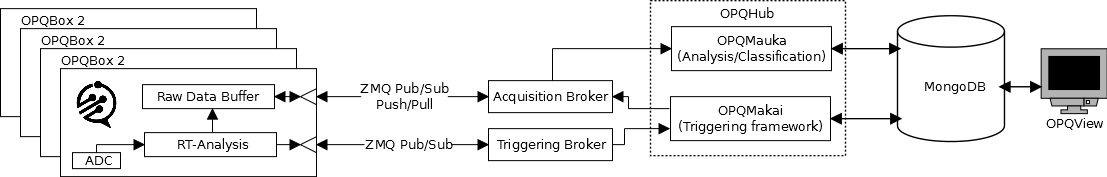
\includegraphics[width=\linewidth]{figures/system-diagram.png}
	\caption{OPQ System Diagram}\label{fig:opq-system}
\end{figure}

\subsubsection{OPQ: Boxes}
An OPQ Box is a custom designed PQ sensor. OPQBoxes can be plugged into a wall outlet and communicate with OPQ servers using the user's WiFi connection. OPQBoxes consist of a Raspberry PI single board computer (SBC), a custom board for PQ measurements, custom firmware, and a custom enclosure. The custom board contains an ADC that samples an alternating current (AC) power signal at 12 thousand samples per second. This data is transferred to the Raspberry Pi where feature extraction and data transfer takes place. The hardware design is presented in figure \ref{fig:opq-box-design} and the software design is provided in figure \ref{}.

\begin{figure}
	\centering
	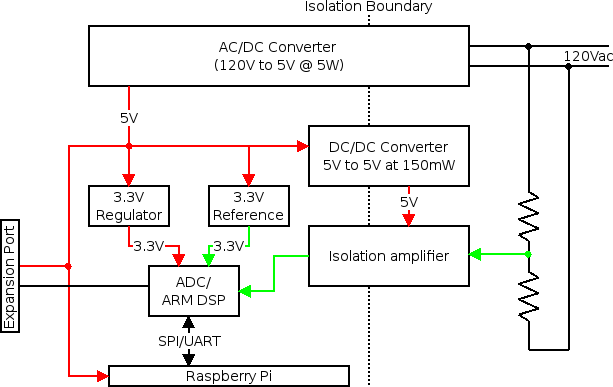
\includegraphics[width=.75\linewidth]{figures/opqbox_diagram.png}
	\caption{OPQ Box Design}\label{fig:opq-box-design}
\end{figure}

\begin{figure}
	\centering
	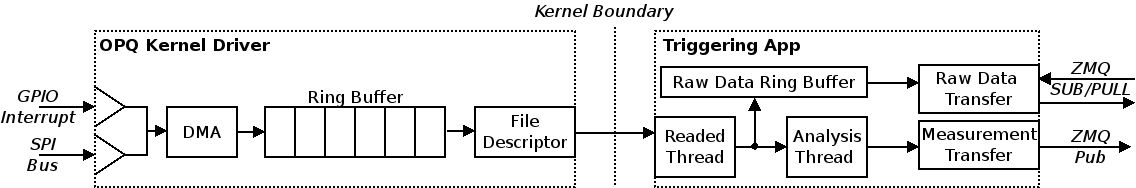
\includegraphics[width=.75\linewidth]{figures/opqbox_software.png}
	\caption{OPQ Box Software}\label{fig:opq-box-software}
\end{figure}

The feature extraction algorithms extract from the sampled waveform the following features: windowed $V_{RMS}$, frequency, and total harmonic distortion (THD) features. The feature extracted data is then sent to a central sink where further analysis is used to determine if the sensor or a subset of sensors should be triggered for raw data.

The OPQ network is a hybrid network that uses edge computing for calculating features at the edge of the network. This is opposed to networks that utilize a ``send everything" approach. In this way, we are able to minimize bandwidth. 

OPQBoxes are synchronized to each other and the OPQ back end using the network time protocol (NTP). This provides synchronization to the millisecond level, which although is great for longer incidents, does not provide accurate timing for transients that may be shorter than tens of milliseconds.


\subsubsection{OPQ: Makai}
OPQ Makai is the central sink and triggering daemon for the OPQ framework. It is made up of several services which are responsible for aggregating and processing the measurements generated by OPQ Boxes. Low fidelity feature extracted data consisting of $V_{RMS}$, frequency, and THD are streamed from OPQ Boxes at a configurable message rate. These data streams are observed by OPQ Makai and the daemon uses statistical methods and thresholds to determine if the sensor or a subset of sensors should be triggered for a window of raw sampled waveforms. 

The OPQMakai system design is provided in figure \ref{fig:makai-main}.

\begin{figure}
	\centering
	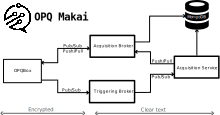
\includegraphics[width=.75\linewidth]{figures/makai_main.pdf}
	\caption{OPQ Makai Design}\label{fig:makai-main}
\end{figure}

\subsubsection{OPQ: Health}
OPQHealth is a service that continuously monitors both the hardware sensors and the software services that make up the OPQ framework.

OPQHealth detects health issues in the following ways. 

OPQHealth determines if an OPQBox is active or inactive by querying the Mongo database for the most recent aggregate measurement. If there is a record of an aggregate measurement within 5 minutes, the Box is considered up, otherwise it is considered down.

The status of OPQMakai is determined by Makai inserting special health events into the Mongo database. Health queries for the presence of these events and if events are not observed within 1 minute, the OPQMakai service is considered down.

OPQMauka provides a special HTTP endpoint that is only accessible within the OPQ back end network that when accessed with a \textit{GET} request will return with a status of \textit{200 OK} if the service is up and available. Any other response of the absence of the response is considered a failure more for OPQMauka.

MongoDB is monitored by querying for a sentinel value that was previously placed in the database.

OPQView is monitored by sending a \textit{GET} request to the landing page. A response of \textit{200 OK} means that the health service is up. Any other response or the lack of response is an indication of failure for OPQView.

OPQHealth stores its findings in both the Mongo database as well as in a traditional log file.

\subsubsection{OPQ: View}
OPQView is a web application that provides visualization, notification, and user management services for data, sensors, and user accounts with the OPQ framework. OPQView is built using Meteor.js and provides a Reactive view of the underlying data stored in the OPQ database.

A screenshot of OPQView in action is provided in figure \ref{fig:opq-view}.
	
\begin{figure}
	\centering
	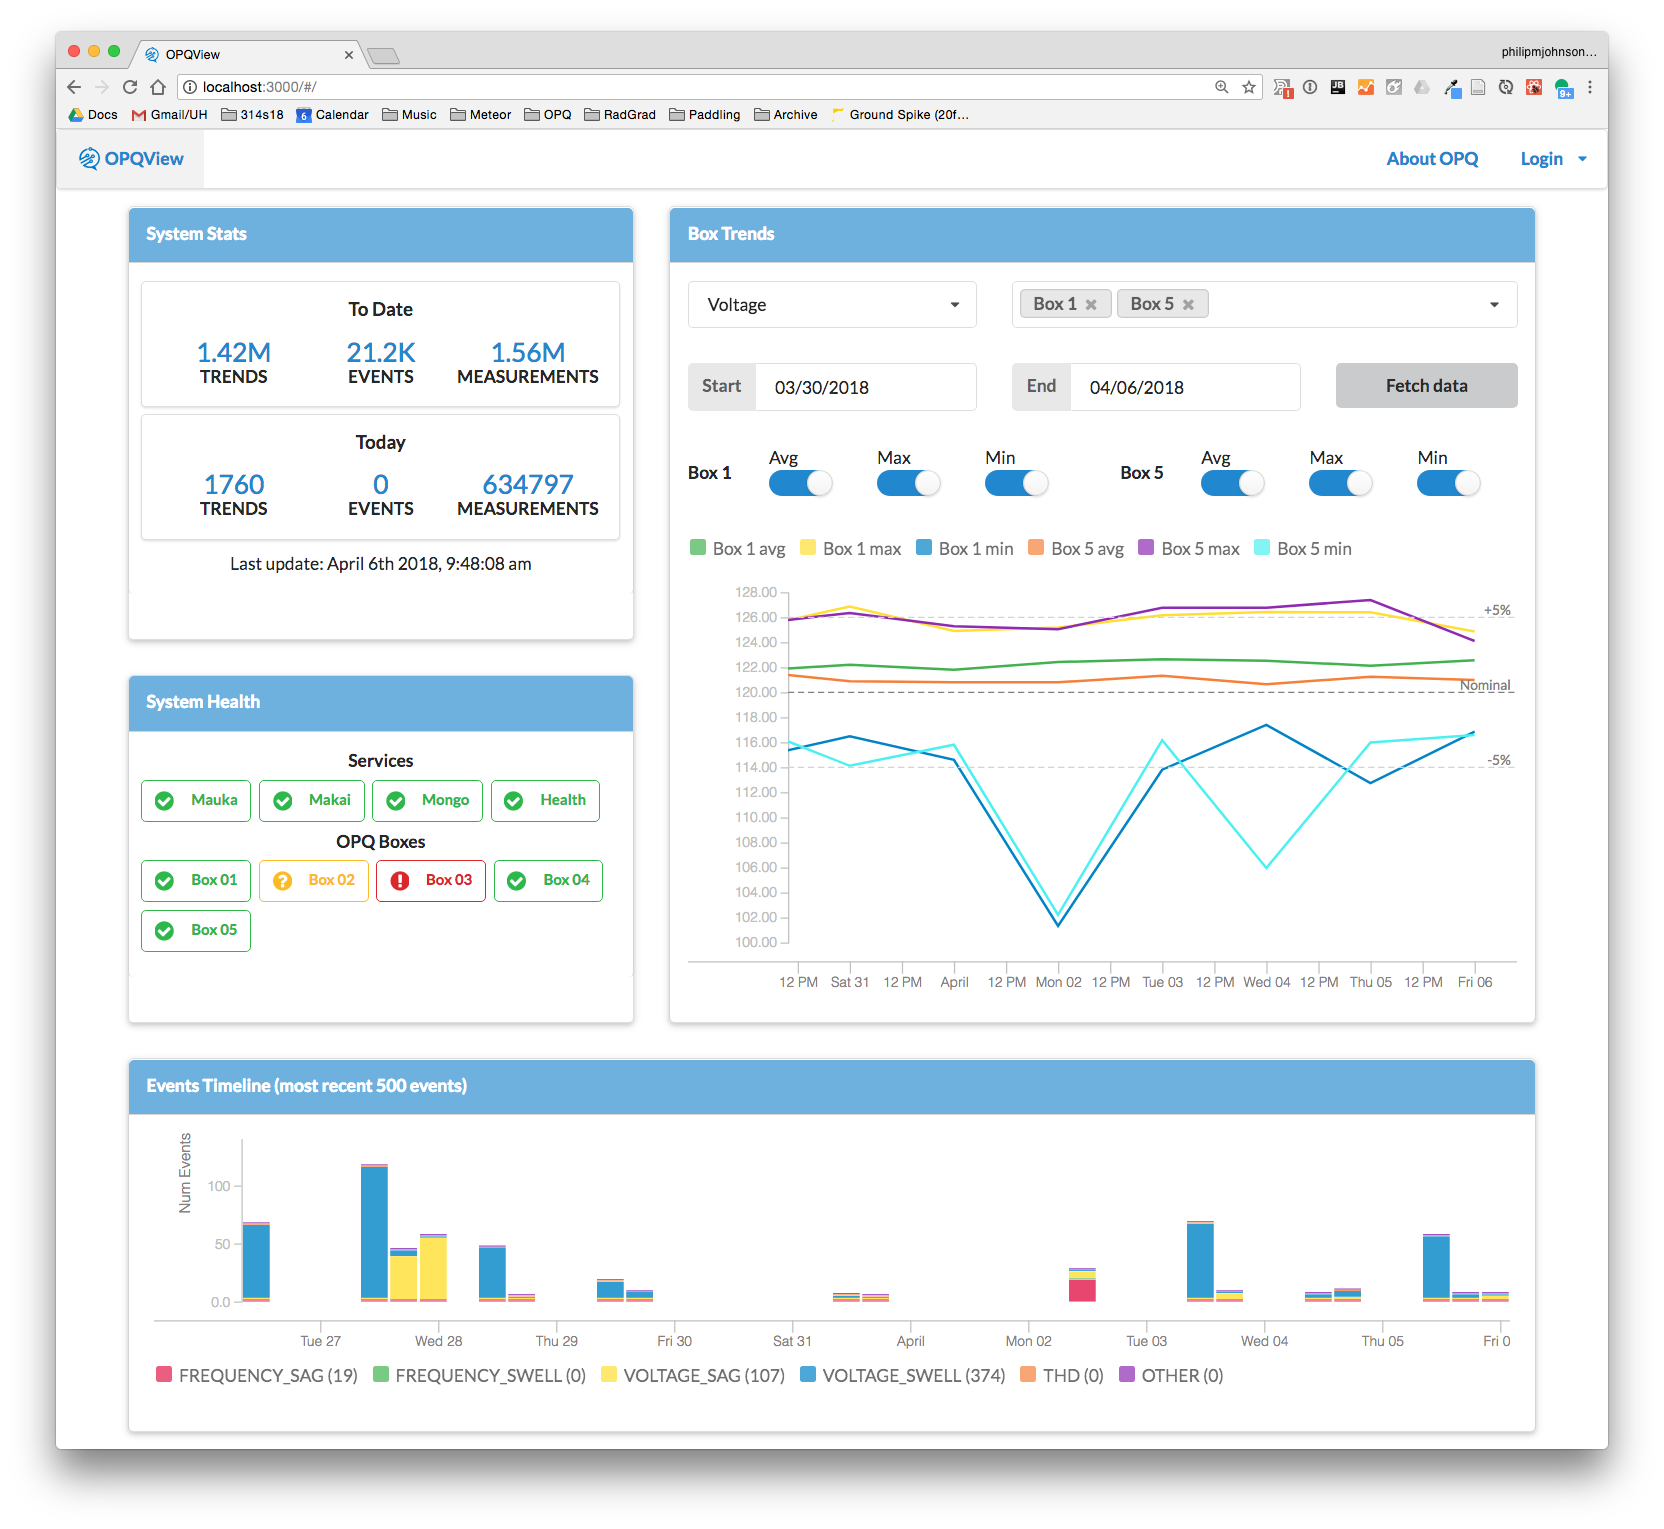
\includegraphics[width=1\linewidth]{figures/opqview-landing-page.png}
	\caption{OPQ View Screenshot}\label{fig:opq-view}
\end{figure}

\subsubsection{OPQ: Mauka}
% TODO

TODO: This section is in the making and will be much more detailed than the other components of OPQ.

\subsubsection{OPQ: Data Model}
% TODO

\subsubsection{OPQ as a Laha-compliant DSN}
% TODO

\subsubsection{Lokahi}
Lokahi is a dynamic DSN that originally evolved as a distributed infrasound detection network. Infrasound is characterized as sound waves that are less than 20 Hz. Infrasound generally can not be deciphered by the human ear, but it can be detected using microphone and barometric pressure sensors. Any large movements of the atmosphere can produce infrasound. The Lokahi network was designed to supplement the International Monitoring System (IMS) for the capture  of undeclared and declared nuclear explosions. Lokahi has been successfully used to capture signals from volcanoes, hurricanes, aircraft, meteors, and other large atmospheric events. 

Sensors in Lokahi are any mobile device that can run iOS or Android. We have sensors distributed world wide. The software stack for Lokahi consists of a distributed actor system for data acquisition, MongoDB for metadata persistence, Apache Kafka for data queues and interprocess communication, Python and related scientific libraries for analysis, and a distributed key-value store for long term storage or sensor data.

Recent development and improvements to the data API have allowed Lokahi to begin accepting data from any of the available onboard sensors on iOS and Android devices. Even though the main focus is still infrasound, having access to all of the available sensors provides the ability to sense other sensor fields and to perform interesting data fusion techniques. 

A diagram of the Lokahi framework is provided in figure \ref{fig:lokahi}.


\begin{figure}
	\centering
	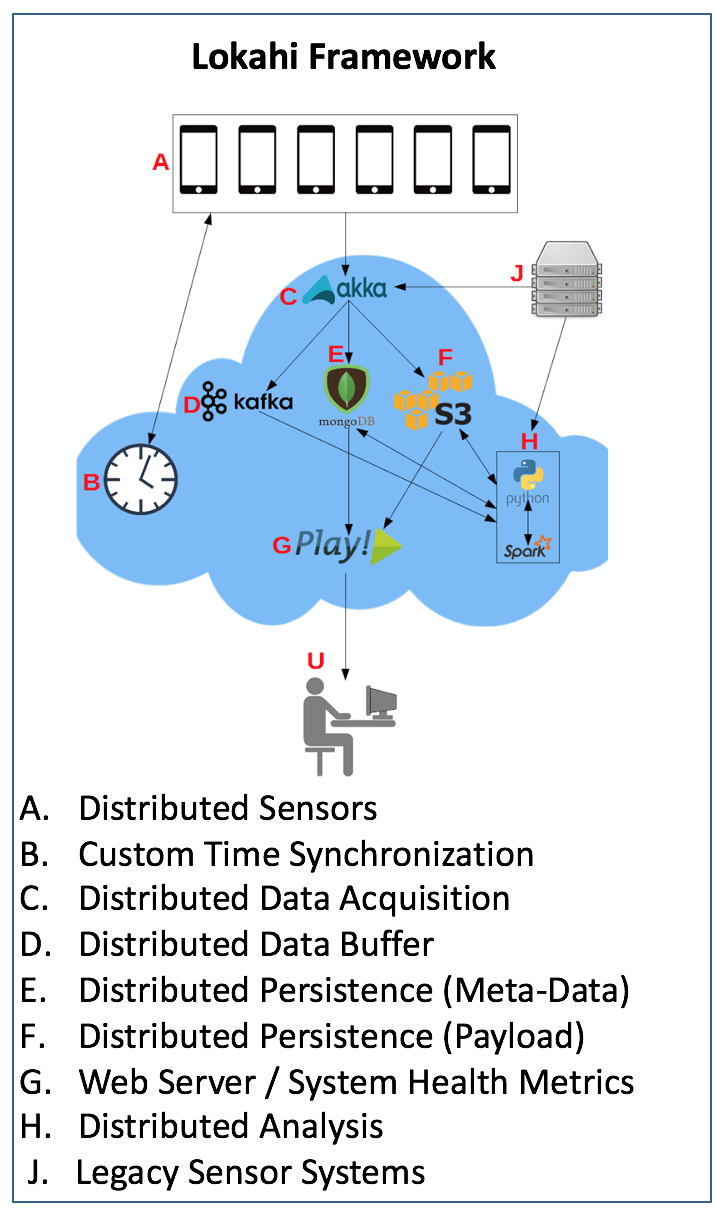
\includegraphics[width=\linewidth]{figures/lokahi.pdf}
	\caption{Lokahi Design}\label{fig:lokahi}
\end{figure}

\subsubsection{Lokahi: Ingestion}
Unlike OPQ, Lokahi takes an approach of send and store everything from every sensor, all the time. This approach is vastly different than what we're used to in triggering based acquisition systems. Data between sensors and our Ingestion servers is encrypted using standard SSL encryption algorithms. Authentication and authorization for each sensor is accomplished using Json Web Tokens (JWTs) with signatures generated using elliptic curve cryptography (ECC). Data at the sensor level is serialized using protocol buffers and then compressed using LZ4. 

To enable the smooth retrieval of large amounts of sensor data, Lokahi uses a distributed actor system (Akka) to automatically scale horizontally based on the current volume of data being received. 

\subsubsection{Lokahi: Persistence}
Metadata is stripped from the sensor data at data ingestion and immediate stored to a distributed Mongo database. Metadata is indexed using a combination of device id and timestamps. 

Metadata drives the rest of the Lokahi framework and provides pointers to the raw data.

Raw sensor data is stored in a distributed key-value store. Lokahi uses Amazon's Simple Storage Service (S3) which provides automatic data redundancy and essentially limitless storage. Raw sensor data is stored by key and the key is stored in the metadata.

Raw sensor data is also persisted in an Apache Kafka queue. Kafka not only provides the framework with a message queue to pass data between distributed services, but it also acts as a ring buffer. Each sensor stores 1 hours worth of data in Kafka that can be looked up by any of the distributed clients and retrieved very quickly. For those reasons, Kafka powers IPC and data buffering roles for our real time analysis of Lokahi sensor data streams.  

\subsubsection{Lokahi: Analysis}
Analysis in Lokahi is provided by a set of distributed processes that were developed in Python using SciPy, NumPy, and matplotlib. Recent developments in the framework are now also including the basis for machine learning (ML) using Tensor Flow.

We provide real time plotting and analysis by subscribing to real time data feeds provided by the Apache Kafka real time queue and buffer. We also provide more robust batch analysis of historical data that can be initiated from Lokahi Web.


\subsubsection{Lokahi: Web}
Lokahi web is a web application for querying and performing analysis of real time sensor data or over historical sensor data. Lokahi also has built in system of health displays for providing a real-time and historic overview of the health of the distributed services within the framework. 

% TODO, provide screenshot

\subsubsection{Lokahi as a Laha-compliant DSN}
%TODO

\subsection{Deploy Laha reference implementations on test sites}
In Q4 2018, 10 to 20 Laha-compliant OPQBoxes will be deployed on the University of Hawaii at Manoa's power microgrid. Using a provided blueprint of the microgrid as a guide and collaborating with the Office of Energy Management, these sensors will be placed strategically with the hopes of observing PQ signals on the same line, PQ signals generated from intermittent renewables, local PQ signals, global PQ signals, and PQ signals near sensitive lab electronics. Many of these sensors will be co-located with industry standard PQ monitoring systems. The industry standard sensors provide both ground truth and a means of comparison between a Laha powered network and a normal DSN. 

In Q4 2018,  20 to 30 Laha-compliant Lokahi sensors will be deployed near and around the Infrasound Laboratory in Kailua-Kona on the Big Island of Hawaii. These sensors will be placed strategically around a calibrated infrasound source. The sensors will be placed with the assistance of Dr. Milton Garces to ensure that we can target sensors at different distances by tuning the amplitude and frequencies of the infrasound signal. In this way, we know which devices should or should not have received the signal.

\subsection{Validate data collected by Laha deployment}
Beginning in Q1 2019, I will begin validated data collection from both the OPQ network and the Lokahi network. 

Data will be validated in the OPQ network be comparing detection and classified signals against industry standard meters that are co-located with our sensors. Data validation will be an autonomous process that validates signals seen in both the industry sensor and the OPQ sensor and also provides a means of quantifying the amount of signals that our sensors were not able to detect. 

Data from the Lokahi network will be validated against industry standard infrasound sensors. We also control the amplitude and frequency of the signals generated from the calibrated infrasound source and can use geophysical equations to predict which sensors should have seen or not seen an infrasonic signal. Data validation is autonomous for this network.

Data validation for both networks will continue for all data collection until the end of the project.

\subsection{Use Laha deployment to evaluate each of the seven proposed benefits discussed in section \ref{laha-benefits}}

\subsubsection{Evaluation of Tiered Management of Big Data}

\subsubsection{Evaluation of Contextualizing Classified Incidents}

\subsubsection{Evaluation of Adaptive Optimizations for Triggering}

\subsubsection{Evaluation of Adaptive Optimizations for Detection and Classifications}

\subsubsection{Evaluation of Model of Underlying Sensor Field Topology}

\subsubsection{Evaluation of Decreased Bandwidth of Entire DSN}

\subsubsection{Evaluation of Decreased Sensor Device Power Requirements of Entire DSN}

\section{Anticipated contributions of this thesis}
\subsection{Laha design: a novel distributed sensor network adaptive design with seven useful properties}
\subsection{Laha evaluation: empirical data to confirm or deny the seven useful properties}
\subsection{OPQMauka and Lokahi: reference implementations of Laha}
\subsection{Implications for modern distributed sensor networks}

\section{Timeline}
\subsection{2018 Q4: Implement, deploy, and validate Laha reference implementations}
\subsection{2019 Q1: Begin validated data collection}
\subsection{2019 Q2: Continue validated data collection, thesis chapters 1-3}
\subsection{2019 Q3: Finish validated data collection, thesis chapters 4-6}






\chapter{Related Work}
This chapter reviews related work looking at defining Big Data in terms of DSNs, Big Data management, self-optimizing DSNs, predictive analytics and forecasting, optimizations to triggering, detection, and classification of signals-of-interest within the context of DSNs.

\section{Big Data and Distributed Sensor Networks}
Big Data is a term that is used to define either the characteristics of collected data or the processes involved for storing and analyzing collected data. Information that is considered Big Data provides a number of challenges.

One of the best and somewhat up-to-date (2014) reviews on Big Data literature is provided by the President’s Council of Advisors on Science and Technology (PCAST) in their report to the White House\cite{house2014big}. In this review, Big Data is described using several definitions. 

The first definition includes ``high-volume, high velocity, and high-variety information assets that demand cost-effective, innovative forms of information processing for enhanced insight and decision making"\cite{gartner_it_glossary_2016}. This definition focuses on the characteristics of the data that make it ``Big". In this context high-volume refers to the total amount of data that requires processing, high-velocity refers to the speed at which data arrives, and high-variety refers to the fact that sensor data is often heterogeneous and incomplete. The second part of the definition includes the terms cost-effective, innovative forms of information processing for enhanced insight and decision processing which hints at the fact that we need technology that is able to deal with these types of data characteristics while doing so within the limits of a system with the goal of refining the data to provide insights and decision making that wouldn't have been possible without the information processing. 

A second definition\cite{ward2013undefined}  mentioned by the PCAST report rings more true to what Laha attempts to accomplish within the context of DSNs and says that Big Data ``a term describing the storage and analysis of large and/or complex data sets using a series of techniques including, but not limited to, NoSQL, MapReduce, and machine learning". This second definition defines Big Data in terms of storage and analysis techniques and is a useful definition for describing the processes by which Laha and the Laha reference DSNs deal with distributed sensor data.

\section{Distributed Sensor Networks and Big Data Management}
There are many technologies for movement, transformation, and storage of sensor data. Current state of the art technologies include distributed streaming and computation engines such as Apache Kafka\cite{kreps2011kafka} or Apache NiFi\cite{noauthor_apache_nodate}. Although these framework provide a lot of flexibility in terms of transformations applied and data management, they do not provide automatic mechanisms for data management. Other, less known technologies are discussed in \cite{hughes2016survey}, but also suffer from the fact that they are flexible in moving large amount of data, but do nothing to address storage requirements or graceful degradation.

Another approach is to use compression techniques, such as those described in \cite{tang2004compression}. However, at scale, even data compression can not keep up with the approach of storing everything all the time.

There are many distributed computation engines and techniques which provide a generic framework for distributing computational tasks across multiple CPUs and multiple machines. The two that are generally receiving the most academic attention are MapReduce\cite{dean2008mapreduce} and Apache Spark\cite{zaharia2016apache}. Although these computation engines are very generic and quite powerful, they can't easily inherit any of the optimizing benefits provided by Phenomena in the Laha framework.

The data grid\cite{chervenak2000data} is a framework that was designed to provide two basic services the authors believe are fundamental for distributed management and analysis of large scientific datasets, storage systems and metadata management. The data grid provides storage abstractions and metadata management with the goal of providing maximum redundancy. That is, the data grid was designed to work with other distributed file systems and computation engines. The data grid also provides control for policy control and privacy safeguards. The data grid does not provide any sort of discarding of data or provide TTL layers for different types of data.

The paper ``Data mining with big data"\cite{wu2014data} constructs the HACE framework which is specifically designed for mining of insightful data from varied Big Data sets. Although this framework is useful for managing multiple streams of data and mining over multiple features, it does not attempt to provide an upper bounds of storage requirements or provide graceful degradation in the face of large scaling networks.

In terms of frameworks using aggregation to facilitate data reduction, Camdoop\cite{costa2012camdoop} is a framework that aims to push aggregation techniques from the edge the entire way to the sink. Camdoop was able to show positive results in data reduction while still maintaining semantic meaning. However, Camdoop was designed to run over simple data streams (such as word count logs) and its not known how this system would perform with more primitive types of data. Camdoop was designed to run within CamCube simulations and its not known how this would run in practice with a real DSN.

\section{Distributed Sensor Networks and Predictive Analytics and Forecasting}
\cite{anastasi_energy_2009} breaks data predictions algorithms for DSNs into two classes. The first class of algorithms are defined as stochastic approaches and use probabilities and statistics to provide predictions. The other class is called time series forecasting and uses historical time series data to provide future predictions. An example of a stochastic model for predicting sensor data is the Ken model\cite{chu2006approximate} which was developed for energy reduction by minimizing the data sent between sensors and sink nodes. This is accomplished by using a model of sensed data and only sending data when the sensed values at the sensor do not match what was predicted by the model. The model is built during a training phase in which a probabilistic density function (PDF) is generated for the model. Ken is flexible enough to provide models for different types of sensed phenomenon and can work anywhere where there are high correlations in time and space.

Time series forecasting algorithms typically use moving average, auto regressive, or auto regressive moving average models. The authors of the PAQ framework\cite{tulone2006paq} uses auto-regression techniques to build a model of sensor readings that is compared between sensor node and sink nodes while  providing probably correct error bounds. The SAF architecture\cite{tulone2006energy}, by the same authors, improves on the PAQ framework by refining the AR models and also adds the ability to not only detect outliers, but also detect inconsistent data. These approaches provide predictions for a single feature, however Laha provides the ability for DSNs to be multi-modal. The paper presented by Le et al.\cite{le2007adaptive} uses time series forecasting, but provides multiple models which are switched out when the data changes. That is, given the current state of the network, a model is selected that is most likely to provide correct predictions. This is useful if a network has multiple features that can be used for forecasting.

\section{Determining Topology and Localization}
The paper by Langendoen and Reijers\cite{langendoen2003distributed} provides comparisons for localization techniques of large DSNs. Langendoen's requires that the approaches are self organizing and do not depend on global infrastructure (such as GPS) , are tolerant to node failures, and are energy efficient. These constraints rule out other localization approaches such as GPS. One thing that differentiates Laha networks to Langendoen's is that Langendoen assumes a random distribution of sensor nodes where sensors in Laha networks are strategically placed. If there are a fraction of nodes that do know their location (anchor nodes), then there are several techniques that meet Langendoen's criteria including Ad hoc Positioning System from Niculescu et al.\cite{niculescu2003ad}, the N-hop Multilateration Primitive by Savvides et al.\cite{savvides2002bits}, and Rabaey's work on robust positioning algorithms\cite{rabaey2002robust}. The three approaches all use three similar phases for localization: distance between anchor nodes and other sensors, position, and refinement. Laha hopes to provide sensor distance between sensors rather than physical distance. The above algorithms use flooding of the network for evaluate distance metrics, which may not be possible in Laha deployed networks.

When timing synchronization between nodes is sufficient, that is, the synchronization between sensors provides a timing accuracy of more than the Nyquist frequency for the signals of interest trying to be captured, it's possible to use arrival time of signals to provide metrics on sensing field topology and localization. This is the premise behind sets of algorithms that look at a single signal and the arrival times of that signal at multiple sensors along with possible direction and then attempt to provide an estimate of source signal localization. This has been performed in infrasound networks using the INFERNO framework as described by Perttu\cite{perttu2013regional} and in other acoustic DSNs such as those used for efficient shooter localization (finding the source of a gun shot from collected acoustic signatures) in \cite{gezici2005localization} and \cite{maroti2004shooter}. Localization of non-acoustic signals has also been shown in the literature. For example, Parsons et al. provide a method for localizing PQ disturbances by analyzing energy flow and peak instantaneous power for both capacitor energizing  and voltage sag disturbances from sampled voltage and current data\cite{parsons1998direction}.

Although not related to determining the topology of a PQ network, there is research that can also find the optimal placement of PQ sensors given a the topology of the network. Won, et al.\cite{won2008optimal} provide an automatic method of placing PQ sensors on a known topology to maximize signal collection while minimizing the total number of required sensors.  

\section{Optimizations for Triggering}
Triggering is the act of observing a feature extracted data stream for interesting features and triggering sensors to provide raw data for a requested time window for higher level analysis. Adaptively optimizing triggering is a way to tune triggering algorithms and parameters with the aim of decreasing false positives and false negatives. In this context, a false positive is triggering on a data stream that does not contain a signal of interest and a false negative is not triggering on a data stream that does contain a signal of interest. 

Many of the optimizing triggering algorithms present in the literature exist to minimize sensor energy requirements and bandwidth requirements. This is addressed in great detail in the literature review by Anastasi et al. \cite{anastasi_energy_2009}. This is accomplished by reducing communications between sensor nodes and the sink. It's argued in \cite{pottie2000wireless} that the cost of transmitting a single bit of information from a sensor cost approximately the same as running 1000 operations on that sensor now. However, there is some contention on this topic as \cite{alippi_adaptive_2010} argues that in some modern sensors computational requirements can equal or eclipse those of  sensor communication.  

One of the main drivers of optimization of triggering is to take advantage of the known sensing field topology of a DSN. This is often referred to in the literature as ``topology control"\cite{santi2005topology}. When the topology of the sensing field is known and when there is an adequate density of sensors, Vuran et al. show that sampled data display strong spatial and temporal correlations\cite{vuran2004spatio}. This fact can be used to reduce the amount of duplicate sensor data that is transmitted, stored, and processed. Topology control is generally split into two categories, ``location  driven" where the location of the sensor is known and ``connectivity driven" which aims to dynamically activate or deactivate sensors to provide complete coverage of a sensing field. Many of the location based approaches in the literature attempt  to maximize the ability for sensors to communicate with each other, however Laha takes the approach that all sensors communicate directly with sink nodes eliminating the need for optimizing intra-sensor communications. One downside to location based approaches is that GPS sensors can be energy hogs and only work with directly line of site to the atmosphere. In these cases, a subset of sensors can be supplied with a GPS and the other sensor use additional techniques such as NTP or statistical analysis to determine location\cite{langendoen2003distributed}.

More details on topology control can be gathered in the reviews by Karl et al.\cite{karl2007protocols} and Vuran et al.\cite{vuran2004spatio}.








\chapter{System Design}
Laha, which means, to spread or distribute in Hawaiian, is an abstract framework for distributed sensor networks that provides a means for big data management as well as augmenting a DSN with the ability to adaptively optimize its bandwidth, detection, classification, and sensor device power requirements.

The Laha framework is made up of five layers that can be viewed conceptually as a pyramid (see \ref{laha-figure}). Data entering the Laha framework is located at the bottom the bottom of the pyramid. As data moves upward through the layers, noise is discarded, less interesting events are discarded or aggregated into upper layers, events are given more meaning and context, and associations and predictions are made. 

\begin{figure}
\caption{Laha Conceptual Model}
\centering
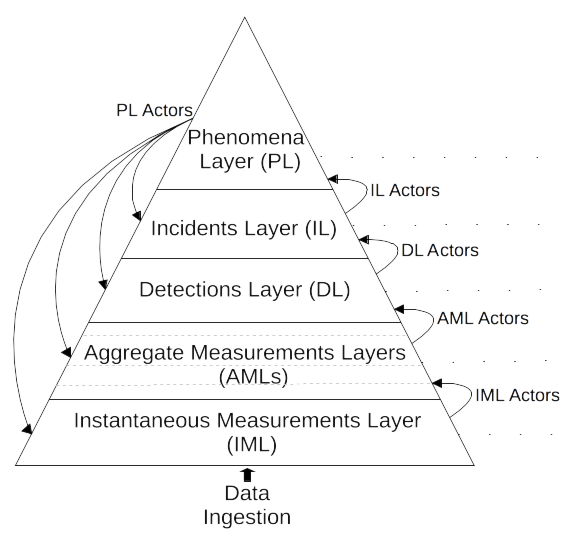
\includegraphics{figures/laha.png}	
\label{laha-figure}
\end{figure}

\section{Five proposed benefits of Laha} \label{laha-benefits}
Laha is designed to adaptively optimize the collection, triggering, detection, and classification of signals within a DSN. These optimizations provide several benefits to DSNs. Many of these benefits can be found in other DSNs, but generally only appear as a single optimization (TODO: CITE) or as a subset of optimizations (TODO: CITE). Laha is the first DSN to combine all of these benefits for the purpose of auto-optimizing the network.

\subsection{Tiered management of Big Data}
% TODO If you're going to use "Big Data" as a term of art, then it needs to be rigorously defined.
% TODO What I think you need to emphasize here is that in any Big Data scenario, you simply can't keep all the data around forever. So, what approach will be used to decide what data to keep and what data to discard?  Laha addresses this problem by having a series of levels, each with its own TTL.  This approach has the benefit of simplifying the analysis of bandwidth and storage requirements for a DSN, but at the cost of potentially discarding important data due to the "use it or lose it" design.  Part of youer evaluation should attempt to address this weakness of use it or lose it.

Laha provides tiered management of the Big Data that the framework consumes. This is mainly accomplished using the layered approach that Laha provides. All data within the Laha framework is garbage collected using a configurable time to live (TTL) for each layer. As data moves from the bottom to the top of the framework, noise is discarded and only interesting data as determined by the higher layers is preserved and forwarded upwards within the framework. In this way, the network can be tuned to preserve increasingly important data. The details of Laha's tiered approach can be found in section \ref{big-data-management}.

\subsection{Automatically provide context to classified incidents}
% TODO This is a feature that will be hopefully much more easily evaluated once you have the two reference implementations.  I will be interested to see what kinds of contextual information are attached, and whether there are times you wished you could attach information elsewhere.
Laha provides Annotations Phenomena (see \ref{annotations-phenomena}) that allows users or algorithms to tag signals of interest with contextual information. There is already a large amount of research for providing classifications of signals of interest, however annotations provide context about the classifications themselves. That is, Laha provides the ability to assign causality to already classified signals.

Initially, a library of annotations is required to be built for a particular DSN. Once the library has been built, Laha can provide automatic annotation assignment using similarity metrics. By using annotations and determining causality, it's possible to create actionable responses to signals observed within a network.

Further, annotations can be used to optimize detection and classification of known signals. For example, imagine a power quality network that observes a voltage sag on the same sensors at the same time periodically. If the cause of the voltage sag can be determined (such as a motor turning on), then detection of this signal can either be muted or analyzed more deeply. Also, other voltage sags that exhibit similar characteristics can then be automatically annotated.

\subsection{Adaptive optimizations for triggering}
% TODO This seems totally cool, but I question whether this is a novel feature. Adaptive setting of thresholds must happen in lots of different domains.  You'll want to discuss related work here, and hopefully argue that other approaches are ad-hoc and domain-specific, but the contribution of Laha is to build adaptive optimization of triggering directly into the framework as a first-class concept. 
Many triggering schemes rely on thresholds being surpassed within feature extracted data streams. For example, triggered data streams in a power quality network might consist of voltage, frequency, and THD extracted features to determine if there is likely a signal of interest observed from a given set of sensors. If any of the extracted features surpass a preset threshold, then we  end up triggering the devices for raw, higher fidelity data. However, there are cases where the feature extracted stream may not surpass a predefined threshold and those sensors would not be triggered.

By using different types of Phenomena, we can improve our triggering efficiency. For example, Locality Phenomena, as discussed in section \ref{locality-phenomena}, allow us to predict detections and classifications in space. If a particular grouping of sensors that are related in space always observe the same detections and classifications, then we can build a predictive model of when the framework can expect to see those things. In this way, a sensor may trigger on a passed threshold, but other sensors that are co-located may not trigger because feature extracted data is below the triggering threshold. If the Locality Phenomena predicts that other co-located sensors should have detected the same signal, then we might trigger those devices for high fidelity data to determine if the signal is in the raw data stream even though it didn't meet the triggering threshold.

Laha can use Periodicity Phenomena, as discussed in section \ref{periodicity-phenomena}, in similar ways. When periodic signals are classified, we can create Future Phenomena that predicts when signals of interest should be detected and classified. This allows Laha to optimize triggering by tuning the triggers to specifically look for Periodic or Future Phenomena. Periodic and Future Phenomena also allows Laha to tune classification algorithms to the predicted classifications.

\subsection{Adaptive optimizations for detection and classification}
Not only can Laha optimize triggering, but similar usages of Locality and Future phenomena can be utilized to improve detection and classification efficiency. With Locality Phenomena, a model of common detections and classifications can be built for a set of co-located sensors. Detection and classification algorithms can be tuned to search for specific signals that are often observed within this model, pruning the search space and increasing the accuracy of detection and classification algorithms.

Future and Periodic Phenomena provide the same benefits to detection and classification as Locality Phenomena. That is, if Laha is able to predict when a signal is going to arrive and also predict how that signal is going to be classified, then it can tune its detection and classification algorithms specifically for the signal of interest.

\subsection{Provides a model of underlying sensor field topology}
% TODO Either this is extremely cool, or totally frivolous, and I'm not sure which. it is frivolous if the only thing it's doing is detecting topology that you already know about (i.e. that two OPQ boxes are close together physically, but we already know that because of their lat/long coordinates.) it is totally cool if you are detecting topology that is not already known. So, it would be good to provide a specific example here for both domains (OPQ and Lokahi)

Predictive phenomena use localization of signals to build communities or groupings of sensors that observe similar signals in both time and space. Over time, Laha can begin to build a model of the underlying topology of the sensing field. For instance, if a group of sensors always see the same signal, then we can assume that either the signal has a far reach, or the sensors are grouped together geographically. With enough sensor penetration, we can differentiate between these two scenarios.

Further, if the sensors provide any sort of location information, Laha can provide a mapping from physical location to sensor field topology. This is especially useful when the topology of the sensor field is not known a priori. Even if we know the location of the sensors at all times, that does not mean that we understand the topology of the sensing field. For example, in a PQ network, the topology is defined by how the electrical grid is connected to itself and laid out. Laha hopes to provide a model that can determine the electrical distance between devices even if the topology of the grid is not known. As another example, take an infrasound network. It's possible that two sensors are located close to each other geographically, but if they have a large mass between them, they may not receive the same signals due to the topology of the environment around them. 

In this sense, Laha is not interested in knowing the location of sensors relative to each other, but is more interested in understanding how signals flow between sensors as a constraint on the topology that the signals travel through.


\subsection{Decreased bandwidth of entire DSN}
One of the tertiary benefits of optimizing triggering and classification is that we get decreased bandwidth usage for free. By improving triggering efficiency, its possible to trigger less devices for raw data when something interesting is observed in the triggering stream.

Predictive phenomena allow us to target triggers to sensors that are most likely to have captured a signal of interest. For instance, if a geographical grouping of sensors tend to always observe the same signals of interest, then we can use that grouping to optimize triggering. Instead of triggering all devices in an area to search for the signal, we can trigger only on the specific grouping that is most likely have observed the signal. We can also selectively ignore sensors within a predictive grouping if Laha assumes that all sensors observed the signal, then we may only need to analyze the signal from one of the sensors rather than all of the sensors in the grouping.

\section{Big Data Management in Laha} \label{big-data-management}
The Laha framework acts as an adaptive sieve for filtering noise and uninteresting data collected from a DSN. In this way, each layer only passes what it considers interesting to the layer above it. All data at a particular layer is garbage collected at specific intervals relating to its important to the DSN.

Each layer only keeps data for a specified amount of time before it is garbage collected. As data moves up the pyramid, it is generally considered more useful and therefore has a longer Time to Live (TTL), the amount of the time the data lives before it is garbage collected.  When a higher layer detects ``something interesting", the data contained in the time window of ``something interesting" is copied into the layers above it and will still persist even though the original data is garbage collected. In this way, we preserve data from all layers if they are associated with interesting data. 

A summary of how data management in Laha is provided in table \ref{data-managament-table}. Note that the TTL is configurable for each implementing network and the table provides default values.

\begin{table}
	\caption{Summary of data management in Laha}
	\begin{tabular}{|c|c|c|}
		\hline 
		Layer & Description & Time-to-Live (TTL) \\ 
		\hline 
		Phenomena Layer (PL) & Contextual \& predictive analytics &  \\ 
		\hline 
		Incidents Layer (IL) & Classified signals &  1 year \\ 
		\hline 
		Detections Layer (DL) & Triggered windowed raw data & 1 week  \\ 
		\hline 
		Aggregate Measurements Layer (AML) & Statistical aggregates of raw data  & 1 day  \\ 
		\hline 
		Instantaneous Measurements Layer (IML) & Raw sensor data  & 1 hour \\ 
		\hline 
	\end{tabular} 
    \label{data-managament-table}
\end{table}

\subsection{Instantaneous Measurements Layer}
The Instantaneous Measurements Layer (IML) receives raw, sampled data from the DSN. The amount of data received is determined by the sample rate of each device multiplied by the number of fields per sample. Most of the time samples, from devices in the network are mainly sampling noise. A large percentage of the data in this layer is destined for garbage collection and data is assigned a Time to Live (TTL) of one hour. 

\subsection{Aggregate Measurements Layer}
The Aggregate Measurements Layer (AML) is responsible for rolling up IMs from the IML. In general, this layer only works with feature extracted data, rather than working with the raw samples. Each measurement in the AML provides summary statistics over a configurable time window. For example, these can include min, max, mean, median, mode, and variance statistics. 

It's possible to breakup the AML into several sub layers, each with different window sizes. For example, we might roll IMs into one minute AMs, then roll one minute AMs into hour AMs, then days, and so on. Each sublayer within the AML can have its own configurable TTL, ensuring long term summary statistics stick around for as long as needed. This provides us a high level view of the network and can provide insights into long term trends which wouldn't be visible (or available) in the IM data stream.

Similar to IMs, AMs can be saved and copied to the layers above it when interesting data is observed. This ability allows for AMs during these time periods to be stored and saved from the garbage collection process.

At this point in the hierarchy, we are still not providing any context to the data that we are receiving. Context is provided by layers above the AML.

\subsection{Detections Layer}
The Detections Layer (DL) is the first layer that provides some context to the data that the sink is receiving. This layer is responsible watching the feature extracted data streams, and requesting IMs from the IM layer. In general, the detection layer is meant to be trigger happy\footnote{Pun intended.} and be overly aggressive when determining if a feature extracted data stream looks interesting. 

When a data stream looks interesting, the DL marks a timestamp $N$ seconds before the interesting features and $M$ seconds after the interesting features, where both $N$ and $M$ are configurable within the framework. The goal is to use a time window that catches signals of interest within it. Since these data ranges will be further processed and refined higher in the hierarchy, there is no issue with collecting larges amounts of data in this layer. 

The actual methods of detection is dependent on the characteristics of every individual sensor network. This framework assumes that the detection algorithms are provided by the implementing frameworks.

Similar to other layers, the DL layer will have its IMs and AMs copied into layers above it when upper layers observe something interesting in the DL. The detections layer is set to have a TTL of a week.

\subsection{Incidents Layer}
Incidents represent classified signals. Incidents are individual classifications for signals of interest and are created by analyzing waveforms from Events. Waveforms from Events may contain multiple incidents. Individual signals may be classified as multiple incidents (for example a transient being classified as both a transient and frequency incidents). 

Incidents are further analyzed to produce phenomena. 

Incidents are expired after one year of storage. 


\subsection{Phenomena Layer}
Phenomena are defined as a grouping of incidents that provide one or more of annotations, locality, periodicity, predictiveness, similarity, and future phenomena. 

Not only do Phenomena provide interesting insight and analytics into the underlying data, but they also provide a means for adaptively tuning the underlying collection, triggering, detection, and analysis of a distributed sensor network.

Phenomena are summarized in table \ref{phenomena-summary-table} and discussed in great detail in section \ref{phenomena}.

\section{Phenomena: Providing Adaptive Optimizations in Laha} \label{phenomena}

\begin{table}
	\centering
	\caption{Summary of Laha Phenomena}
	\begin{tabular}{|c|c|}
		\hline
		Phenomena & Description \\
		\hline
		Annotations & Provide context about an Incident or set of incidents \\
		\hline
		Locality & Provides context on how incidents are related in time and space \\
		\hline
		Periodicity & Designation for incidents that exhibit repetitive or periodic behavior \\ 
		\hline
		Similarity & Subset of incidents found using grouping and community detection algorithms \\
		\hline
		Predictive & Subset of incidents characterized by predictive or forecasting models\\
		\hline
		Future & Incidents scheduled to occur in the future\\
		\hline
	\end{tabular}
	\label{phenomena-summary-table}
\end{table}

\subsection{Annotations Phenomena} \label{annotations-phenomena}
Annotations provide context about an Incident or a set of Incidents. Annotations are generally user provided or sourced from other data sources to provide supporting context to Incidents. For example, Annotations might include “Cloud Cover”, “Hurricane Hector”, “Dryer Turns On”, etc.

In some sense, annotations allow us to label our data sets beyond a simple classification and start looking at causal classifications. Once enough annotations have been assigned to classified incidents, Laha can used Annotations to attempt to label unknown incidents with similar characteristics.

Annotations can be used to tune Laha's detection and classification algorithms by allowing Laha to filter on incidents with known causes.

\subsection{Locality Phenomena} \label{locality-phenomena}
Locality provides context on how incidents are related to each other in both space in time. Laha is able to determine if classified incidents are local to a single sensor, to a group of co-located sensors, or global across an entire network. Sensors can be co-located in both the physical sense and also co-located within a sensing field. For example, sensors in a power quality network may be separated by large distance geographically, but co-located through the electrical grid and the grid's topology. 

Over time, Locality Phenomena is used to build a model of sensors in relation to each other and to provide a statistical likelihood that co-located sensors will observe the same signal. Locality phenomena can be used to drive network triggering, detection, and classification thresholds within a distributed sensor network by using this probabilistic model for determining the likelihood that a sensor or sensors will observe a signal of interest.

\subsection{Periodicity Phenomena} \label{periodicity-phenomena}
Periodic phenomena consists of incidents that exhibit repetitive behavior, that is, the same types of incidents appearing in cycles from single or multiple devices. Periodicity allows for the easy creation of Predictive phenomena.

Periodic phenomena can come from a single incident or from multiple incidents. Periodic phenomena allow us to either tune our network to find periodic incidents or tune the  network to ignore periodic incidents depending on if the incidents are of interest. Periodic phenomena are especially useful in conjunction with Annotation phenomena as we can assign causality to the periodic signal. 

\subsection{Similarity Phenomena}
Similarity phenomena utilize grouping and community detection algorithms to group incidents together by their features. Common features used for grouping include time, location, incident type, or incident features.

% TODO describe common community detection algorithms 

\subsection{Predictive Phenomena}
Predictive phenomena consists of incidents that are characterized by a predictive or forecasting models. Predictiveness is a behavior that can be inferred from all other phenomena types. 

Predictiveness is the main driver behind optimizing the control of a distributed sensor network. If we can predict the types of signals that will arrive at sensors, then we can tune those sensors and the sink to either filter the signals (if the user is not interested in signals) or tune the sensors and the sink to be extra sensitive to those signals, possible detecting them even if they previously would not have been detected.

\subsection{Future Phenomena}
Predictive phenomena can be used to create future phenomena. Future phenomena are a statistical model of the likelihood of seeing an incident or incidents at future points in time. Knowing that a signal may occur with some probability allows agents affected by those signals time to prepare for the signals.

\section{Laha Actors: Acting on the Laha Data Model}
Laha Actors act on the Laha hierarchy and provide one of two functions. Actors can move data from one level of the hierarchy upwards through the hierarchy when interesting data is requested by an upper level. Actors can also apply adaptive optimizations downwards through the hierarchy. The Laha framework can support multiple actors at each level. For example, the Incidents Layer in our reference power quality network contains actors for each of the following functions: IEEE classified voltage events, frequency variations, power outages, excessive THD, and many others. The Incident Layer Actors move data from these incidents upwards to the Phenomena Layer.  

Table \ref{laha-actors-tables} summarizes the actors that exist within the Laha framework and their purposes. 

\begin{table}
	\centering
	\caption{Summary of Laha Actors}
	\begin{tabular}{|c|c|}
		\hline
		Actor & Purpose \\
		\hline
		IML Actors & Perform feature extraction and move aggregate data to AML \\
		\hline
		AML Actors & Perform triggering on data from IML, copy data to DL if interesting \\
		\hline
		DL Actors & Perform high fidelity feature extraction on possible detections \\
		\hline
		IL Actors & Perform classification and contextualization on possible detections \\
		\hline
		PL Actors & Generate predictive analytics and optimize the lower levels of the hierarchy \\
		\hline
	\end{tabular}
	\label{laha-actors-tables}
\end{table}

\subsection{Actor Constraints}
Actors at each level in the hierarchy are governed by a set of constraints. These constraints include the set of possible inputs, $A_i$, the set of possible outputs, $A_o$, the set of Actors it can receive data from, $A_{ai}$, the set of Actors it can transmit data to, $A_{ao}$, and a set of performance metrics that each actor must maintain, $A_p$. The constraints assigned to each Actor are determined by the hierarchy level in which the Actor resides.  

Actors are responsible for reporting constraint violations and in this way, Actors are the primary provider of health, performance, and status metrics about the Laha framework.

The constraints for each level of Laha hierarchy is summarized in table \ref{actor-constraint-table}.

\begin{table}
	\centering
	\caption{Summary of Laha Actor Constraints at Each Level}
	\begin{tabular}{|c|c|c|c|c|c|}
		\hline
		Level & $A_i$ & $Ao$ & $A_{ai}$ & $A_{ao}$ & $A_p$ \\
		\hline
		IML & Raw samples & Aggregate trends & n/a & AML & Data ranges available \\
		\hline
		AML & Aggregate trends & Detections & IML & DL & Data ranges available \\
		\hline
		DL & Windowed waveforms & Hi-fi extracted features & AML & IL & Data \& features available \\
		\hline
		IL & Hi-fi extracted features & Contextualized incidents & DL & PL & Incident types available \\
		\hline
		PL & Contextualized incidents & Optimizations & IL & All levels & Optimizations available \\
		\hline
	\end{tabular}
	\label{actor-constraint-table}
\end{table}

\section{OPQ: A Laha-compliant Power Quality DSN}
OPQMauka is a middleware component of the Open Power Quality (OPQ) framework. The OPQ project provides a hardware and software solution for monitoring distributed power quality (PQ). The OPQ project was founded with the goal of studying how intermittent distributed renewable energy sources affect PQ not just at a user's home, but also within a user's neighborhood, between neighborhoods, and globally across the grid. 

The OPQ ecosystem is made up of networked hardware sensors (OPQBoxes) and various software services (OPQMakai, OPQMauka OPQHealth, OPQView). Each of these software components are made up of individual services and plugins.

The OPQ system design is laid out in figure \ref{fig:opq-system}.

\begin{figure}
	\centering
	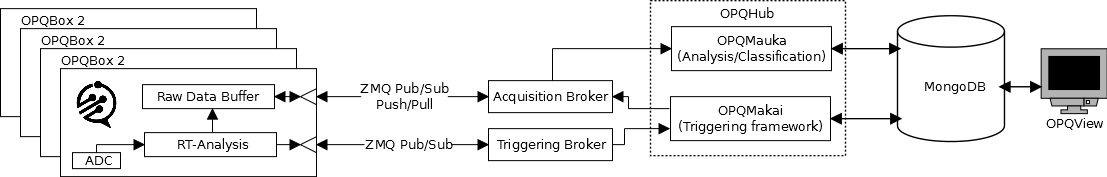
\includegraphics[width=\linewidth]{figures/system-diagram.png}
	\caption{OPQ System Diagram}\label{fig:opq-system}
\end{figure}

\subsection{OPQ: Boxes}
An OPQ Box is a custom designed PQ sensor. OPQBoxes can be plugged into a wall outlet and communicate with OPQ servers using the user's WiFi connection. OPQBoxes consist of a Raspberry PI single board computer (SBC), a custom board for PQ measurements, custom firmware, and a custom enclosure. The custom board contains an ADC that samples an alternating current (AC) power signal at 12 thousand samples per second. This data is transferred to the Raspberry Pi where feature extraction and data transfer takes place. The hardware design is presented in figure \ref{fig:opq-box-design} and the software design is provided in figure \ref{}.

\begin{figure}
	\centering
	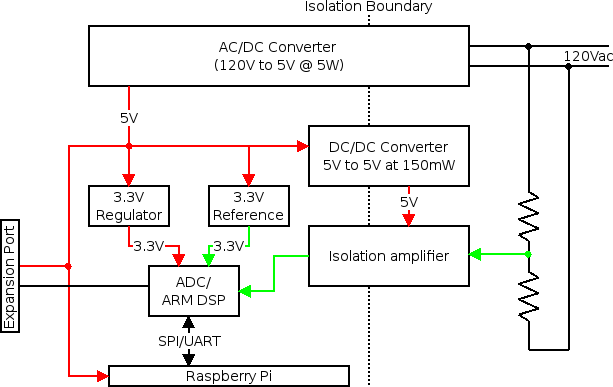
\includegraphics[width=.75\linewidth]{figures/opqbox_diagram.png}
	\caption{OPQ Box Design}\label{fig:opq-box-design}
\end{figure}

\begin{figure}
	\centering
	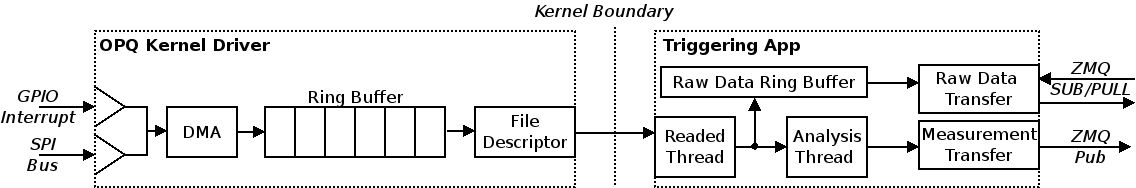
\includegraphics[width=.75\linewidth]{figures/opqbox_software.png}
	\caption{OPQ Box Software}\label{fig:opq-box-software}
\end{figure}

The feature extraction algorithms extract from the sampled waveform the following features: windowed $V_{RMS}$, frequency, and total harmonic distortion (THD) features. The feature extracted data is then sent to a central sink where further analysis is used to determine if the sensor or a subset of sensors should be triggered for raw data.

The OPQ network is a hybrid network that uses edge computing for calculating features at the edge of the network. This is opposed to networks that utilize a ``send everything" approach. In this way, we are able to minimize bandwidth. 

OPQBoxes are synchronized to each other and the OPQ back end using the network time protocol (NTP). This provides synchronization to the millisecond level, which although is great for longer incidents, does not provide accurate timing for transients that may be shorter than tens of milliseconds.


\subsection{OPQ: Makai}
OPQ Makai is the central sink and triggering daemon for the OPQ framework. It is made up of several services which are responsible for aggregating and processing the measurements generated by OPQ Boxes. Low fidelity feature extracted data consisting of $V_{RMS}$, frequency, and THD are streamed from OPQ Boxes at a configurable message rate. These data streams are observed by OPQ Makai and the daemon uses statistical methods and thresholds to determine if the sensor or a subset of sensors should be triggered for a window of raw sampled waveforms. 

The OPQMakai system design is provided in figure \ref{fig:makai-main}.

\begin{figure}
	\centering
	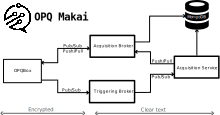
\includegraphics[width=.75\linewidth]{figures/makai_main.pdf}
	\caption{OPQ Makai Design}\label{fig:makai-main}
\end{figure}

\subsection{OPQ: Health}
OPQHealth is a service that continuously monitors both the hardware sensors and the software services that make up the OPQ framework.

OPQHealth detects health issues in the following ways. 

OPQHealth determines if an OPQBox is active or inactive by querying the Mongo database for the most recent aggregate measurement. If there is a record of an aggregate measurement within 5 minutes, the Box is considered up, otherwise it is considered down.

The status of OPQMakai is determined by Makai inserting special health events into the Mongo database. Health queries for the presence of these events and if events are not observed within 1 minute, the OPQMakai service is considered down.

OPQMauka provides a special HTTP endpoint that is only accessible within the OPQ back end network that when accessed with a \textit{GET} request will return with a status of \textit{200 OK} if the service is up and available. Any other response of the absence of the response is considered a failure more for OPQMauka.

MongoDB is monitored by querying for a sentinel value that was previously placed in the database.

OPQView is monitored by sending a \textit{GET} request to the landing page. A response of \textit{200 OK} means that the health service is up. Any other response or the lack of response is an indication of failure for OPQView.

OPQHealth stores its findings in both the Mongo database as well as in a traditional log file.

\subsection{OPQ: View}
OPQView is a web application that provides visualization, notification, and user management services for data, sensors, and user accounts with the OPQ framework. OPQView is built using Meteor.js and provides a Reactive view of the underlying data stored in the OPQ database.

A screenshot of OPQView in action is provided in figure \ref{fig:opq-view}.

\begin{figure}
	\centering
	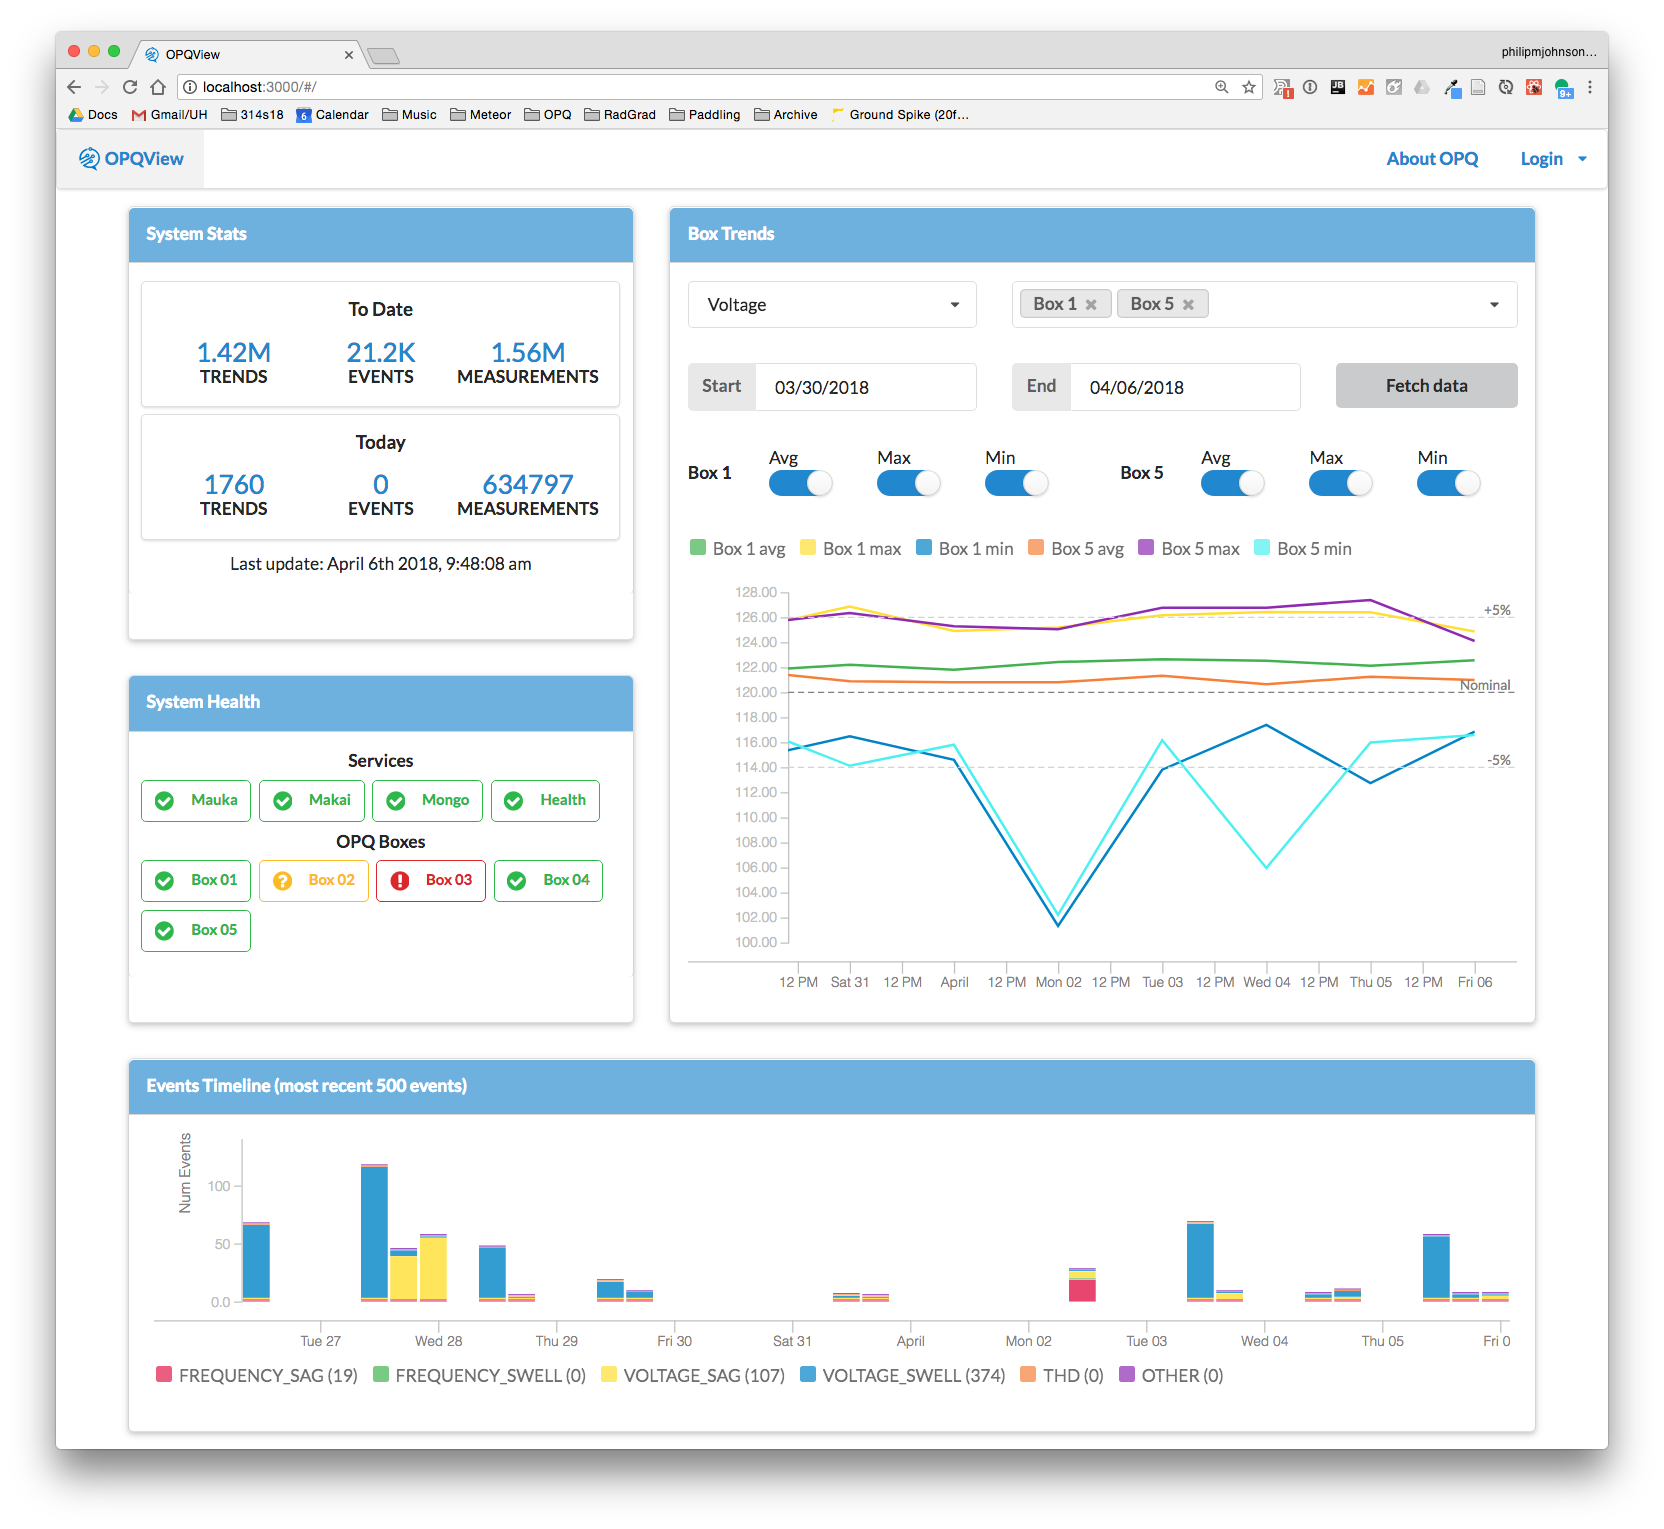
\includegraphics[width=1\linewidth]{figures/opqview-landing-page.png}
	\caption{OPQ View Screenshot}\label{fig:opq-view}
\end{figure}

\subsection{OPQ: Mauka}
% TODO

TODO: This section is in the making and will be much more detailed than the other components of OPQ.

\subsection{OPQ: Data Model}
% TODO

\subsection{OPQ as a Laha-compliant DSN}
OPQ and specifically OPQMauka comply with the Laha abstract framework. Table \ref{opq-compliance} summarizes how the OPQ data architecture fits within the Laha conceptual model.

\begin{table}
	\caption{OPQ as a Laha-compliant DSN}
	\begin{tabular}{|c|c|c|c|c|}
		\hline 
		Laha Layer & OPQ & Created By & Stored By & TTL \\ 
		\hline 
		IML & raw ADC Samples & OPQBox & Onboard memory & 20 minutes \\ 
		\hline 
		AML & min,max,avg V, F, THD & OPQBox & trends\footnotemark & 1 day \\ 
		\hline 	
		DL & triggered waveforms & Makai/Mauka & events/box\_events\textsuperscript{\ref{fn-1}} & 1 week \\
		\hline
		IL & Classified detections & Mauka & incidents\textsuperscript{\ref{fn-1}} & 1 year \\
		\hline
		PL & Predictive analytics & Mauka & phenomena\textsuperscript{\ref{fn-1}} & N/A \\
		\hline
	\end{tabular}
	\label{opq-compliance}
\end{table}  
\footnotetext{MongoDB Collection Name\label{fn-1}}

In order to be a Laha compliant DSN, the reference DSN must also implement Laha Actors. Table \ref{opq-actors} summarizes how OPQ implements Laha actors.

\begin{table}
	\caption{OPQ  Actors Implementation}
	\begin{tabular}{|c|c|c|}
		\hline 
		Laha Actors & OPQ Equivalent & Description \\ 
		\hline
		IML Actors & Boxes & Store window of raw sensor samples \\
		\hline
		AML Actors & Boxes \& Makai & Makai stores and triggers on aggregate data from Boxes \\
		\hline
		DL Actors & Mauka & MakaiEvent plugin \\
		\hline
		IL Actors & Mauka & Voltage, Frequency, THD, Outage, plugins \\
		\hline
		PL Actors & Mauka & Annotations, Locality, Similarity,  Periodic, Predictive,  Future plugins\\
		\hline
	\end{tabular}
	\label{opq-actors}
\end{table}  

\section{Lokahi: A Laha-compliant Infrasound DSN}
Lokahi is a dynamic DSN that originally evolved as a distributed infrasound detection network. Infrasound is characterized as sound waves that are less than 20 Hz. Infrasound generally can not be deciphered by the human ear, but it can be detected using microphone and barometric pressure sensors. Any large movements of the atmosphere can produce infrasound. The Lokahi network was designed to supplement the International Monitoring System (IMS) for the capture  of undeclared and declared nuclear explosions. Lokahi has been successfully used to capture signals from volcanoes, hurricanes, aircraft, meteors, and other large atmospheric events. 

Sensors in Lokahi are any mobile device that can run iOS or Android. We have sensors distributed world wide. The software stack for Lokahi consists of a distributed actor system for data acquisition, MongoDB for metadata persistence, Apache Kafka for data queues and interprocess communication, Python and related scientific libraries for analysis, and a distributed key-value store for long term storage or sensor data.

Recent development and improvements to the data API have allowed Lokahi to begin accepting data from any of the available onboard sensors on iOS and Android devices. Even though the main focus is still infrasound, having access to all of the available sensors provides the ability to sense other sensor fields and to perform interesting data fusion techniques. 

A diagram of the Lokahi framework is provided in figure \ref{fig:lokahi}.


\begin{figure}
	\centering
	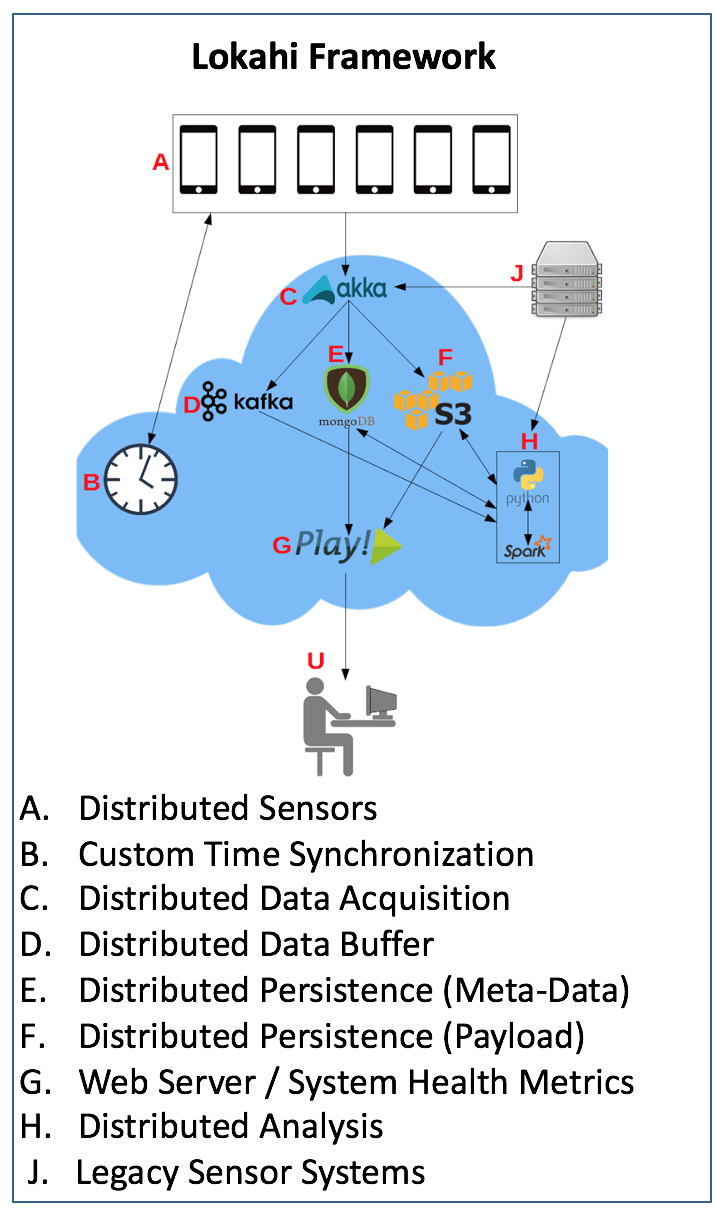
\includegraphics[width=\linewidth]{figures/lokahi.pdf}
	\caption{Lokahi Design}\label{fig:lokahi}
\end{figure}

\subsubsection{Lokahi: Ingestion}
Unlike OPQ, Lokahi takes an approach of send and store everything from every sensor, all the time. This approach is vastly different than what we're used to in triggering based acquisition systems. Data between sensors and our Ingestion servers is encrypted using standard SSL encryption algorithms. Authentication and authorization for each sensor is accomplished using Json Web Tokens (JWTs) with signatures generated using elliptic curve cryptography (ECC). Data at the sensor level is serialized using protocol buffers and then compressed using LZ4. 

To enable the smooth retrieval of large amounts of sensor data, Lokahi uses a distributed actor system (Akka) to automatically scale horizontally based on the current volume of data being received. 

\subsubsection{Lokahi: Persistence}
Metadata is stripped from the sensor data at data ingestion and immediate stored to a distributed Mongo database. Metadata is indexed using a combination of device id and timestamps. 

Metadata drives the rest of the Lokahi framework and provides pointers to the raw data.

Raw sensor data is stored in a distributed key-value store. Lokahi uses Amazon's Simple Storage Service (S3) which provides automatic data redundancy and essentially limitless storage. Raw sensor data is stored by key and the key is stored in the metadata.

Raw sensor data is also persisted in an Apache Kafka queue. Kafka not only provides the framework with a message queue to pass data between distributed services, but it also acts as a ring buffer. Each sensor stores 1 hours worth of data in Kafka that can be looked up by any of the distributed clients and retrieved very quickly. For those reasons, Kafka powers IPC and data buffering roles for our real time analysis of Lokahi sensor data streams.  

\subsubsection{Lokahi: Analysis}
Analysis in Lokahi is provided by a set of distributed processes that were developed in Python using SciPy, NumPy, and matplotlib. Recent developments in the framework are now also including the basis for machine learning (ML) using Tensor Flow.

We provide real time plotting and analysis by subscribing to real time data feeds provided by the Apache Kafka real time queue and buffer. We also provide more robust batch analysis of historical data that can be initiated from Lokahi Web.


\subsubsection{Lokahi: Web}
Lokahi web is a web application for querying and performing analysis of real time sensor data or over historical sensor data. Lokahi also has built in system of health displays for providing a real-time and historic overview of the health of the distributed services within the framework. 

% TODO, provide screenshot

\subsubsection{Lokahi as a Laha-compliant DSN}
TODO
\chapter{Evaluation}
Evaluation of the Laha framework involves deploying reference Laha-compliant DSNs, validating the data collected from the reference implementations, and then comparing and contrasting various metrics for each of the proposed goals. Metrics will be collected during a set of experiments for each of the Laha reference implementations in early 2019. 

The following sections describe my plans for deployment of reference implementations, data validation, evaluating the main goals of the Laha framework, and evaluating the tertiary goals of the Laha framework.

\section{Deploy Laha reference implementations on test sites}
In Q4 2018, 10 to 20 Laha-compliant OPQBoxes will be deployed on the University of Hawaii at Manoa's power microgrid. Using a provided blueprint of the microgrid as a guide and collaborating with the Office of Energy Management, these sensors will be placed strategically with the hopes of observing PQ signals on the same line, PQ signals generated from intermittent renewables, local PQ signals, global PQ signals, and PQ signals near sensitive lab electronics. Many of these sensors will be co-located with industry standard PQ monitoring systems. The industry standard sensors provide both ground truth and a means of comparison between a Laha designed network and a non-Laha designed network.. 

In Q4 2018,  20 to 30 Laha-compliant Lokahi sensors will be deployed near and around the Infrasound Laboratory in Kailua-Kona on the Big Island of Hawaii. These sensors will be placed strategically around a calibrated infrasound source. The sensors will be placed with the assistance of Dr. Milton Garces to ensure that I can target sensors at different distances by tuning the amplitude and frequencies of the infrasound signal. In this way, I know which devices should or should not have received the signal.

\section{Validate data collected by Laha deployment}
Beginning in Q1 2019, I will begin validated data collection from both the OPQ network and the Lokahi network. 

Data will be validated in the OPQ network be comparing detected and classified signals against industry standard meters that are co-located with our sensors. Data validation will be an autonomous process that validates signals and trends seen in both the industry sensor and the OPQ sensors. Data validation will provide metrics for signals and trends that the reference sensors observed but OPQ sensors did not (false negatives) as well as signals that the OPQ sensors observed and the reference sensors did not (false negatives).  Specifically, I will be looking to compare long term trends (voltage, frequency, and THD readings over a time period of days) as well as more transient signals of interest (i.e. voltage sags/swells, frequency variations, excessive THD, and outages).

Data from the Lokahi network will be validated against industry standard infrasound sensors. We also control the amplitude and frequency of the signals generated from the calibrated infrasound source and can use geophysical equations to predict which sensors should have seen or not seen an infrasonic signal. Data validation is autonomous for this network as well. Similar to the OPQ network, I will be collecting metrics on false positive and false negatives as compared to the reference sensors. 

Data validation for both networks will continue for all data collection until the end of the project.

\section{Use Laha deployments to evaluate the main goals of the framework}
The Laha deployments for both OPQ and Lokahi will be used to evaluate each of the main goals this framework claims to provide. Namely that Laha is a generally useful framework representation for DSNs. Second, Laha provides the ability to turn primitive sensor data into actionable data and insights. Third, Laha's tiered management of sensor data provides metrics on maximum bounds for storage requirements and graceful degradation of DSN performance. 

Each deployment offers different techniques for performing evaluation. 

In the OPQ deployment, OPQBoxes are deployed and co-located with industry standard, calibrated, reference sensors. Each of these sensors cost thousands to obtain and install, collect all the data all the time, and can only be connected to the power main as it enters a building. These sensors provide a means for verifying signals received or not received by OPQ, as well as confirming long term trend data. I have been provided access to these sensors and stored data via the Office of Energy Management at UH Manoa. The data is accessible via an HTTP API. The Office of Energy Management at UH Manoa has also provided the full schematics for the UH power grid. This will be used as a ground truth for topology estimates and distributed signal analysis. OPQBoxes are placed in strategic locations on the UH Manoa campus specifically in order to evaluate the distributed nature of PQ signals. For example, OPQBoxes are placed on the same electrical lines as well as separate electrical lines to observe how PQ signals travel through an electrical grid.

In the Lokahi deployment, I have the opportunity to generate infrasound signals using a calibrated infrasound source \cite{park2009rotary}.. The source can be tuned to produce infrasound at configurable frequencies and amplitudes. The source works by attaching a variable pitch propeller to an electric motor that can be driven by a waveform generator. The source can generate signals that can be observed at large stand off distances, over tens of kilometers. Similar to the OPQ deployment, sensors within the Lokahi deployment will be co-located with industry standard, calibrated, infrasound sensors. These sensors can provide a metric of signals that were correctly observed, incorrectly observed, or not observed at all by the Lokahi deployment. Further, infrasound itself is characterized quite well by various geophysical equations. These equations can be used to predict if sensors deployed in the Lokahi deployment are likely to observe generated infrasound signals.

Evaluation of the main goals of this network are provided in the following sections.

\subsection{Evaluation of the Generality of this Framework}
I claim that the Laha framework is useful and general enough to be applied to DSNs in different domains. To test this, I will design, develop, and deploy two DSNs. The first OPQ, measures distributed PQ signals on the electrical grid. The second, Lokahi, observes infrasound signals traveling through the atmosphere. 

To evaluate the generality of the Laha design, I will provide metrics for whether or not each deployment is able to fulfill the goals of the given network.

I expect the PQ network, OPQ, to be able to detect and classify common PQ issues. I expect OPQ to observe voltage dips, voltages swells, frequency dips, frequency swells, transients, and high levels of THD. A count of these signals will be kept and compared against industry standard PQ meters co-located with each sensor. By comparing these signals to the ground truth, we will be able to tabulate a number of false positives and false negatives. In order to be considered effective, I would expect to be able to classify each of these common PQ signals, collect a set of each of the PQ signals while maintaining a low number of false positives and false negatives as compared to the industry standard sensors. In general, a negative result here would be not being able to detect PQ signals of a specific type or having a high number of false positives or false negatives.

Further, another stated goal of OPQ is to detect and classify distributed PQ incidents. That is, PQ signals that are observed by more than one sensor in situations where OPQ sensors are not co-located. First, I will evaluate if OPQ is capable of detecting distributed PQ signals. I expect OPQ to at least observe one distributed signal during the test deployment, but would not be surprised to see many. By working with the Office for Energy Management at UH Manoa, I will use a list of known PQ source events along with signals collected by OPQ and the industry standard sensors to provide a list of false positives and false negatives for the number of distributed PQ incidents observed by OPQ.

I expect the infrasound network, Lokahi, to be able to securely detect and report on infrasound incidents from a large collection of heterogeneous smartphone based infrasound sensors. This network prioritizes availability and security even in the face of network issues or no network at all. I claim that Laha is a useful framework for a DSN such as this and will evaluate if Laha is able to meet the goals of this network.

To evaluate the effectiveness of Laha as implemented by Lokahi, I will deploy 50 heterogeneous Lokahi smartphone sensors at predetermined distances from a calibrated infrasound source. I will then use the calibrated infrasound source to generate infrasound signals of different amplitudes and frequencies. While signals are being generated, I will disable network access for the sensors to simulate real life network drop outs of sensors. I will disable the networks for time periods of 1 minute, 30 minutes, and 1 hour. 

I will then, for each sensor, calculate the number of false positives and false negatives for detections of infrasound signals. In order for Laha to be a useful framework for Lokahi, Lokahi must demonstrate that not only can it detect infrasound signals at different frequencies and amplitudes, but it must also do this while maintaining a low number of false positives or false negatives. 

Further, as availability is a major priority of this network, network outages must be handled without signal loss. To evaluate this goal, I will measure the amount of false negatives (or missed signals) due to Laha's data management and the interplay with network outages. I would expect that if Lokahi implements it correctly, we should not see a rise in false negatives. A less great result would be an increase in false negatives.

Finally, backed by the metrics for both deployments, I will provide a critical discussion on what types of DSNs Laha is well suited for and what types of DSNs Laha is not well suited for. This will include a discussion on which parts of the Laha design are useful or a detriment to a given goal of the DSN.

The following sections continue to discuss the evaluation strategies required to show that Laha is a generally useful representation for a DSN.

\subsection{Evaluation of Converting Primitive Data into Actionable Insights}
An important goal of any DSN is to convert primitive sensor data into actionable insights. This is generally accomplished by adding some kind of context associated with the data such as classifications of a signal or linking the data with other data by comparing similarities in time, space, or other physical features.

I claim that Laha's use of Actors acting on and moving data between levels in the Laha hierarchy provides a useful and generic approach to systematically adding context to data as it moves through the framework. Laha is designed with a specific number of levels where data within each level shares the same type. In each deployment, I will evaluate the usefulness of each level with regards to adding context to the data.

In both deployments, I will evaluate the number of false negatives for incident classification. Each level in the framework is responsible for not only adding context, but deciding if data should be moved upward through the levels, adding more context along the way, or discarding data because a level does not think the data is ``interesting". I will keep track of the number of false negatives and which level was responsible for discarding the data with the signal. Using this approach, I will evaluate the effectiveness of each level to determine which levels correctly identify signals and which levels do not correctly identify signals, thus discarding the data.

In order to be useful, I expect each level to add context to the data while maintaining a low level of false negatives.

Using these metrics, I will provide a discussion on which domains a leveled approach may work well for versus which domains a leveled approach might not provide useful benefits.

I claim that Laha is able to provide even more context and actionable insights by implementing a level called Phenomena. Phenomena utilize predictive analytics to provide context and actionable insights over the sensor domain. First, I will evaluate if Phenomena take place in practice for both of the Laha deployments. 

To evaluate Phenomena in the OPQ network, OPQ must observe a cyclical incident such as voltage swells occurring every afternoon due to solar output or an electric motor turning on at the same time every day. Once a cyclical incident is observed, OPQ must correctly create predictive Phenomena that predict the same incident happening in the future. Assuming predictive Phenomena are created, I will measure the amount of false positives and false negatives on whether the predictions were correct or not. A positive result would show that now only is OPQ capable of making predictive Phenomena, but also that a high percentage (> 50\%) of the predictions are correct.

Evaluation of predictive Phenomena in the Lokahi infrasound network will follow a similar strategy. However, since I can control the infrasound source, I can actually run an experiment that creates cyclical and non-cyclical signals. I will then test Lokahi's ability to not only create predictive Phenomena, but also show that the predictions are accurate, that is, greater than 50\% of them are correct. 

A negative result would be that if either of the networks are not able to create predictive Phenomena or a large number of false positives or false negatives (combining for <50\% prediction accuracy).

Adding context to classified Incidents is the act of providing a statistical likelihood of the underlying cause of the Incident. These include things like showing that a voltage sag is caused by turning on the dryer every day at 2PM or an identifying as infrasound signal as a repetitive flight pattern near an airport. Context is provided by external sources to the DSN (such as users or by performing data fusion with other correlating data sets).

Evaluating contextualized events consists of setting up experiments where I assign context for a specific set of signals and resulting Incidents. Then testing to see if Phenomena are able to correctly apply context to Incidents when the same signals are generated again. I will record the number of false positives and false negatives for assigning context to Incidents.

A positive result would be to see the correct context applied to incidents more than half of the time. That is, I expect context to be applied correctly to at more than 50\% of Incidents for which context has been previously defined.

I expect to see contextualization work better in DSNs where signals provide more measures for discrimination. For example, PQ networks contain many different types of classified PQ signals, however there is a small subset of causes attributed to each type of PQ signal classification.This decreases Laha's search space and in theory should make it easier to provide context.

\subsection{Evaluation of Tiered Management of Big Data}\label{eval-big-data}
The goal of tiered management of Big Data is to add a mechanism that provides a maximum bounds on storage requirements of sensor data at each level in the Laha hierarchy while simultaneously reducing sensor noise as Laha Actors move ``interesting" data upwards. This in turn should decrease the amount of false positives since forwarded data is more likely to include signals of interest and less likely to be sensor noise. 

Other approaches to Big Data management include compression\cite{tang2004compression} or storage systems where the goal is to have a distributed file system and move data close to where it is being processed, such as the Hadoop Distributed File System\cite{warrier2007much}. Other systems such as NiFi\cite{hughes2016survey} provide a nice interface for ingestion and movement of data between Big Data tools while also providing data provenance, but do not go far enough in focusing on data reduction and graceful degradation. Carney et al.\cite{carney2002monitoring} discuss how monitoring applications require management and clean up of stale sensor data.

It's not yet to be seen if I will see a decrease in false negatives. On the one hand, it's possible that Laha will throw away data that did contain signals of interest. In this case, detection or classification Actors will not observe the signals because the data has been discarded leading to increased false negatives. On the other hand, by reducing false positives and increasing the signal-to-noise ratio as data moves upward, Phenomena has a better chance of optimizing triggering, detection, and classification which may in turn inform Laha to save data that would have been previously thrown away. In this way, it's possible that Laha will reduce false negatives.

We will evaluate the number of false positives and false negatives in detections, classifications, and Phenomena compared against industry standard reference sensors. A positive outcome for this metric would be a reduction in both false positives and false negatives compared to an approach that does not use tiered data management. A negative result would be an increase in either false positives or false negatives. 

During the acquisition and curating of data, metrics will be collected and stored about how much data is saved (in bytes) versus how much data is discarded at each level within the Laha data hierarchy. These numbers will be compared against data storage as if the OPQ and Lokahi frameworks were to take a ``store everything" approach. Evaluation metrics provided will include percentage of data storage saved per data hierarchy level as well as an estimate of overall decrease in data storage requirements for the entire DSN. A positive result from these metrics would show significant reduction in storage requirements for each level in the framework compared against a ``store everything approach" and other state-of-the-art data storage solutions.

I will also provide metrics on ``continuous storage pressure" which is a measure of the average amount of data storage required at each level given the current state of the network. That is, since data at all lower levels of the framework assigns a TTL to the data within the collection, the collection will exhibit a constant data pressure during sensor data collection. For example, at the lowest level, the IML collects raw data from all sensors all the time. Given the sample rate per sensor, the size per sample, the number of sensors, and a known TTL for this level, I can estimate the maximum bounds of data management requirements that the IML requires. We can play similar estimation games with higher levels of the framework. I will compute the statistical error between the predicted storage pressure and the actual storage pressure recorded during the experiments. A positive outcome would show strong correlation between the predicted storage pressure and the actual storage pressure. A negative outcome would show weak correlation between the predicted and actual values.

Finally, I will provide an evaluation that weighs the results of all three metrics against each other. For example, if I see positive results for data storage reduction and negative results for false positives, do the benefits of the data storage reduction outweigh the negatives of increased false positives?

I would expect that DSNs that have a lower signal-to-noise ratio will see greater benefits from tiered data management than DSNs that already have a decent signal-to-noise ratio.

\section{Evaluation of Tertiary Goals}
In order to achieve the main goals of this framework, I claim that either all or a subset of the following tertiary goals must be fulfilled. Optimization of triggering, detection, classification, sensor energy usage, bandwidth, predictive analytics, and the ability to derive models of the underlying sensing field topology. 

To evaluate these tertiary goals, I will select and implement DSN optimization techniques from current literature. I will then compare and contrast the usefulness of different techniques and discuss how each of these techniques perform in the different sensor domains.

Finally, I will discuss how each of these tertiary goals make progress towards overall goals of this sensor network.

\subsection{Evaluation of Adaptive Optimizations for Triggering}
Triggering is the act of observing a feature extracted data stream for interesting features and triggering sensors to provide raw data for a requested time window for higher level analysis. Adaptively optimizing triggering is a way to tune triggering algorithms and parameters with the aim of decreasing false positives and false negatives. In this context, a false positive is triggering on a data stream that does not contain a signal of interest and a false negative is not triggering on a data stream that does contain a signal of interest. 

Adaptive triggering is only useful in networks that utilize triggering. Specifically, this technique can not be applied to DSNs that take a collect everything all the time approach.

Triggering can also have significant impacts on overall sensor power requirements and DSN bandwidth requirements. Many of the optimizing triggering algorithms present in the literature exist to minimize sensor energy requirements and bandwidth requirements. This is addressed in great detail in the literature review by Anastasi et al. \cite{anastasi_energy_2009}. This is accomplished by reducing communications between sensor nodes and the sink. It's argued in \cite{pottie2000wireless} that the cost of transmitting a single bit of information from a sensor cost approximately the same as running 1000 operations on that sensor now. However, there is some contention on this topic as \cite{alippi_adaptive_2010} argues that in some modern sensors computational requirements can equal or eclipse those of  sensor communication.  

Even if a DSN utilizes triggering, it's not clear that adaptive triggering even takes place. The first question I will evaluate is, does adaptive optimization of triggering take place at all given the domain of the DSN? That is, does the nature of the underlying sensor field contribute to optimization of triggering? I will compare if and how optimizations take place in the two reference networks for the domains of PQ and infrasound.

In order to evaluate triggering efficiency within our Laha deployments, Laha will only adaptively modify triggering for half of the devices in the OPQ deployment. In the Lokahi deployment, I will run the same experiment twice. The first run will not optimize triggering and the second run will optimize triggering.

Once the experiments have been run, I will first determine if optimization of triggering has occurred, and if it did, compare the number of false negatives and false positives against the runs that did not use optimized triggering or where optimization did not occur. 

I hope to show that a side effect of Laha's optimized triggering is reduced bandwidth and sensor energy requirements. To this end, I will calculate metrics for total data sent and received at the sink node of each network for each device in the network. A positive result would show decreased bandwidth usage for devices that utilize optimized triggering. A negative result would show similar or more bandwidth usage for devices that utilize optimized triggering.

I further hope to show that another benefit of Laha's optimized triggering is reduced sensor energy requirements. The evaluation for this metric will occur with the Lokahi network where sensors can be dependent on batteries. I will run two experiments. For each experiment, all sensors will be charged to battery level of 100\%. In the first experiment, I will not utilize optimized triggering. In the second experiment I will utilize optimized triggering. In both experiments, I will measure the final battery level after the experiment and also measure how quickly the battery depletes for each sensor. This is possible because data in the Lokahi network contains timestamped entries with battery levels.

\subsection{Evaluation of Adaptive Optimizations for Detection and Classifications}
Detections occur when triggering observes something ``interesting" in the feature extracted data stream. A Detection is a contiguous window of raw sensor data that was requested by triggering that may or may not contain signals of interest. Optimizing detections involves optimized the window sizes to increase the signal-to-noise ratio of the window. Fine grained features are then computed by Detection Actors and moved to the Incidents Level where classification of signals takes place. Optimizing Detections involves trimming detection windows to increase signal-to-noise. Optimizing of classifications for Incidents involves tuning parameter sets for the underlying classification algorithms. 

Predictive and Locality Phenomena as well as topology optimizations will be used to provide optimizations to the Detections and Incidents levels. 

Evaluation of adaptive optimizations for detection and classification within the Laha network will be conducted differently for each Laha deployment.

In the Lokahi deployment, I will control the production of infrasound signals using the available infrasound source. I will run two experiments, where the amplitudes and frequencies of the signals are the same and the locations of the devices remain invariant. In the first experiment, Laha will not use optimized detection or classification provided by Phenomena. In the second experiment, Laha will use optimized detection and classification techniques provided by Phenomena. 

With known frequencies and amplitudes of the infrasound signals, I can compare the rate of detections and classifications between the optimized and unoptimized experimental runs. I expect to see a greater number of and more accurate detections and classifications from the optimized experiment.

In the OPQ deployment, I will compare the same metrics as the Lokahi deployment, but instead of controlling the source signal, I will co-locate OPQBoxes. In each pair of co-located OPQBoxes, one will be analyzed using Phenomena optimized detection and classification algorithms and the other will be analyzed using unoptimized detection and classification algorithms.

I will collect and evaluate the number of false positives and false negatives for Incidents generated with optimization and without optimization. A positive outcome would include a decrease in either false positives, false negatives, or both. A negative result would be an increase in either or both false positives or false negatives.

I will also calculate the signal-to-noise ration in Detections to determine if optimization of detections is working. A positive outcome would be an increase in the signal-to-noise ration and a negative outcome would be similar or a decrease in signal-to-noise ratio.

\subsection{Evaluation of Model of Underlying Sensor Field Topology}
Laha hopes to build a model of the underlying sensing field topology. This is not the topology of the physical layout of the sensors (this is generally already known a priori or by collecting location information), but rather the topology by which signals travel. For example, in a PQ network the topology is the physical power grid and switches that PQ signals travel through. In an infrasound network, the topology is the atmosphere through which sound waves travel. Laha aims to build a statistical model of the distances between sensors according to the topology of the sensing field by observing recurrent incidents over time. This can perhaps shed some light on understanding the topology of a sensing field without knowing anything about it before hand.

Much of the literature on topology management is written to decrease sensor energy requirements by exploiting the density of sensors within a sensing field topology. For example, the ASCENT\cite{cerpa2004ascent} framework provides adaptive self configuring sensors that exploit topology denseness to decrease sensor energy usage. Several other frameworks have been designed with the same goal of reducing energy usage by exploiting topology\cite{schurgers2002stem},\cite{schurgers2002topology}.

To evaluate the model of the sensing field topology, I will take two different approaches for each Laha deployment. In both deployment, the sensing field topology is known beforehand to provide a ground truth. I will then compare Laha's computed signal distance between sensors to the actual signal distance between sensors as provided by the ground truths.

In the Lokahi deployment, sensors will be strategically placed at different distances from an infrasound source. Some sensors will be close to each other geographically, but separated by terrain that infrasound signals will not easily travel through. By moving the infrasound source, I can expect to see infrasound signals arriving or not arriving at the sensors depending on the source and direction of the signal along with the physical features of the land. By performing multiple experiments, I hope to provide a model of the physical environment topology that Laha has built. I will compare Laha's model to the known topology and provide a statistical error analysis. 

In the OPQ deployment, sensors will be strategically placed on like and unlike electrical lines to observe how distributed PQ signals move through a power grid. In this deployment, Laha will build a topology model that doesn't show physical geographic distance between sensors, but instead will build a model of the electrical distance between sensors. This data will be evaluated by comparing the electrical distances found by the Laha model to the actual UH power grid as referenced by the schematic provided by the Office of Energy Management at UH Manoa. A statistical error analysis of the differences between electrical distances between the model and the schematic will be provided as an evaluation metric.

A positive outcome would be to show that there is high correlation between the Laha signal distances and the ground truth distances. A negative outcome would show low correlation.

Assuming high correlation and a statistical model of the sensing field, I would like to evaluate if Laha is able to use this information to optimize triggering, classification, or predictive analytics. In order to evaluate this, I will collect the number of false positives and false negatives at all levels in the Laha hierarchy while optimizing from topology and without optimizing from topology. I expect to see less false positives and less false negatives when utilizing topology optimizations. A negative result would be a larger number of false positives or false negatives.

I expect to only see results in networks where signals travel fast enough to create a statistical difference between arrival times at the various sensors. In sensing fields where signals travel slowly and uniformly (i.e. a temperature collection DSN), it may be more difficult or impossible to actually determine the sensing field topology.

%\chapter{Conclusions}

Here is where you discuss your conclusions and future directions.

%%% Switch to appendix mode
%\appendix

%%% Bring in any appendices from external file (optional)
%%%%%%%%%%%%%%%%%%%%%%%%%%%%%%% -*- Mode: Latex -*- %%%%%%%%%%%%%%%%%%%%%%%%%%%%
%% uhtest-appendix.tex -- 
%% Author          : Robert Brewer
%% Created On      : Fri Oct  2 16:31:12 1998
%% Last Modified By: Robert Brewer
%% Last Modified On: Mon Oct  5 14:41:05 1998
%% RCS: $Id: uhtest-appendix.tex,v 1.1 1998/10/06 02:07:03 rbrewer Exp $
%%%%%%%%%%%%%%%%%%%%%%%%%%%%%%%%%%%%%%%%%%%%%%%%%%%%%%%%%%%%%%%%%%%%%%%%%%%%%%%
%%   Copyright (C) 1998 Robert Brewer
%%%%%%%%%%%%%%%%%%%%%%%%%%%%%%%%%%%%%%%%%%%%%%%%%%%%%%%%%%%%%%%%%%%%%%%%%%%%%%%
%% 

\chapter{Some Ancillary Stuff}

Ancillary material should be put in appendices, which appear before the
bibliography. 

\chapter{More Ancillary Stuff}

Subsequent chapters are labeled with letters of the alphabet.


%% Just for demo purposes, include all entries from bib file
%\nocite{*}

%%% Input file for bibliography
\bibliography{references}
%% Use this for an alphabetically organized bibliography
\bibliographystyle{plain}
%% Use this for a reference order organized bibliography
%\bibliographystyle{unsrt}

\end{document}
